\makeatletter
\def\input@path{{./AcceptTest/}}
\makeatother

% Dokumentklassen sættes til memoir.
% Manual: http://ctan.org/tex-archive/macros/latex/contrib/memoir/memman.pdf
\documentclass[a4paper,11pt,oneside,article]{memoir}
\setlrmarginsandblock{*}{2.5cm}{0.75} % højre og venstre 
\setulmarginsandblock{3cm}{*}{1.2} % top og bund 
\checkandfixthelayout[nearest] % specifikt valg af højde algoritme
 
% Danske udtryk (fx figur og tabel) samt dansk orddeling og fonte med
% danske tegn. Hvis LaTeX brokker sig over æ, ø og å skal du udskifte
% "utf8" med "latin1" eller "applemac". 
\usepackage[utf8]{inputenc}
\usepackage[danish]{babel}
\usepackage[T1]{fontenc}
\usepackage{mflogo}

%sexy pdf'er
%\usepackage[export]{adjustbox}
\usepackage{pdfpages}
\usepackage{pdflscape}

%Kompakte lister
\usepackage{paralist}
 
% Matematisk udtryk, fede symboler, theoremer og fancy ting (fx kædebrøker)
\usepackage{amsmath,amssymb}
\usepackage{bm}
\usepackage{amsthm}
\usepackage{mathtools}
\parindent=0pt 

% Fancy ting med enheder og datatabeller. Læs manualen til pakken
% Manual: http://www.ctan.org/tex-archive/macros/latex/contrib/siunitx/siunitx.pdf
\usepackage{siunitx}
 
% Indsættelse af grafik.
\usepackage{graphicx} 
\usepackage{fix-cm} 
\usepackage{soul}
\sodef\an{}{0.13em}{0em}{0em} \sodef\ann{}{0.13em}{0.5em}{0em}
 
%Fancy tabeller.
%\usepackage[table]{xcolor}
\usepackage{multirow}
\usepackage{rotating} %sidewaystables!
\usepackage{longtable} %tables spanning multible pages.
\usepackage{tablefootnote} %for at indstætte fornoter i tabeller.
\usepackage{hhline} %Fixer farvede felter
\usepackage{ltxtable} %Longtabular X
\usepackage{tabularx} %Med dynamisk bredte

%URL fodnoter
\usepackage{url}

% Reaktionsskemaer. Læs manualen for at se eksempler.
% Manual: http://www.ctan.org/tex-archive/macros/latex/contrib/mhchem/mhchem.pdf
\usepackage[version=3]{mhchem}

%Lav chapter clickable og fjern border
\usepackage{hyperref}
\hypersetup{
    colorlinks,
    citecolor=black,
    filecolor=black,
    linkcolor=black,
    urlcolor=black
}

%Table of contents settings
\setsecnumdepth{subsection} % organisational level that receives a numbers
\settocdepth{subsection}   % print table of  for level 3

%Til programkode
\usepackage{listings}
\usepackage{color}

\definecolor{dkgreen}{rgb}{0,0.6,0}
\definecolor{gray}{rgb}{0.5,0.5,0.5}
\definecolor{mauve}{rgb}{0.58,0,0.82}
 
\lstset{ 
  language=C++,                % the language of the code
  basicstyle=\footnotesize,           % the size of the fonts that are used for the code
  numbers=left,                   % where to put the line-numbers
  numberstyle=\tiny\color{gray},  % the style that is used for the line-numbers
  stepnumber=1,                   % the step between two line-numbers. If it's 1, each line 
                                  % will be numbered
  numbersep=5pt,                  % how far the line-numbers are from the code
  backgroundcolor=\color{white},      % choose the background color. You must add \usepackage{color}
  showspaces=false,               % show spaces adding particular underscores
  showstringspaces=false,         % underline spaces within strings
  showtabs=false,                 % show tabs within strings adding particular underscores
  frame=single,                   % adds a frame around the code
  rulecolor=\color{black},        % if not set, the frame-color may be changed on line-breaks within not-black text (e.g. commens (green here))
  tabsize=2,                      % sets default tabsize to 2 spaces
  captionpos=b,                   % sets the caption-position to bottom
  breaklines=true,                % sets automatic line breaking
  breakatwhitespace=false,        % sets if automatic breaks should only happen at whitespace
  title=\lstname,                   % show the filename of files included with \lstinputlisting;
                                  % also try caption instead of title
  keywordstyle=\color{blue},          % keyword style
  commentstyle=\color{dkgreen},       % comment style
  stringstyle=\color{mauve},         % string literal style
  escapeinside={\%*}{*)},            % if you want to add LaTeX within your code
  morekeywords={*,...}               % if you want to add more keywords to the set
}

%Til at udregne forskel mellem sider, brug \pagedifference{A}{B} mellem to labels A og B.
\usepackage{refcount}
\newcommand{\pagedifference}[2]{%
  \number\numexpr\getpagerefnumber{#2}-\getpagerefnumber{#1}\relax}
 
%Til at lave referencer med:
\usepackage{cite}

%Til at lave eksterne \ref til \labels
\usepackage{xr}

%Forsøg på nice lister i tabeller
\usepackage[shortlabels]{enumitem}

\newenvironment{packed_enum}{
\begin{enumerate}[1., topsep=0pt, nosep, partopsep=0pt, parskip=0pt, itemsep=0pt, parsep=0pt]
}{\end{enumerate}}

\newenvironment{packed_item}{
\begin{itemize}[•, topsep=0pt, nosep, partopsep=0pt, itemsep=0pt, parsep=0pt]
}{\end{itemize}}


\title{Home Automation System \\ Gruppe 1}
\author{ 2. Semesterprojekt E2PRJ2-03 \\ Ingeniørhøjskolen, Aarhus Universitet \\ Vejleder: Arne Justesen}
\date{17. december 2014}

%Så man kan hive samtlige \labels i projektdokumentationen, alle har prefix "P-"
\externaldocument[P-]{../Projektdokumentation/main}

\begin{document}
\frontmatter
\maketitle
\begin{table} [h]
	\centering
	\begin{tabular}{|l|r|l|}
	\hline 
	\textbf{Navn} & \textbf{Studienummer} & \textbf{Underskrift~~~~~~~~~~~~~~~~~~~~} \\ \hline
	Morten Hasseriis Gormsen & 201370948 & \\ && \\ \hline
	Kristian Thomsen & 201311478 & \\ && \\ \hline
	Philip Krogh-Pedersen & 201311473 & \\ && \\ \hline
	Lasse Barner Sivertsen & 201371048 & \\ && \\ \hline
	Henrik Bagger Jensen & 201304157 & \\ && \\ \hline
	David Erik Jensen & 11229 & \\ && \\ \hline
	Kasper Torp Samuelsen & 201311498 & \\ && \\ \hline
	Kristian Søgaard Sørensen & 20115255 & \\ && \\ \hline
	\end{tabular}
\end{table}

\newpage

\chapter{Resumé}
Denne rapport omhandler et 2. semesterprojekt på Ingeniørhøjskolen, Aarhus Universitet på retningerne Elektro, IKT og stærkstrøm. Projektarbejdet omhandler design og implementering af et Home Automation System, der kan simulere tilstedeværelse i en bolig for at forebygge indbrud. 

Tilstedeværelse simuleres ved at forskellige elektriske enheder i hjemmet tændes og slukkes automatisk, så en evt. indbrudstyv foranlediges til at tro, at der er nogen hjemme. 

Systemet styres fra en PC, der kommunikerer serielt med en central transmitter controller. Transmitter controlleren anvender herefter X.10 protokol til, via elnettet, at kommunikere med receiver controllere, som bl.a. tænder og slukker de tilkoblede elektriske enheder. 

Software til PC og microcontrollere er skrevet i C++, hardware er testet på fumlebræt og implementeret på simple veroboard. Som controllere er anvendt Atmel STK500 udviklingskit monteret med ATMega32 microcontrollers. Systemet indeholder desuden en kodelås implementeret på DE2-board.

Systembeskrivelsen indeholder flere funktioner (styring af radio og TV), end der er implementeret. Den del af systemet, der er implementeret, kan tænde og slukke to forskellige LED'er samt dimme disse i trin á $10\%$. 

Under projektarbejdet er der anvendt tilpassede udgaver af V-model, ASE-modellen, Scrum og SysML til styring af arbejdet. 

Med undtagelse af en enkelt del af dimmefunktionen, fungerer det implementerede system fuldstændig upåklageligt.
\chapter{Abstract}
This document is about a second semester project at Aarhus University, School of engineering, for students studying electrical-, computer science- and high voltage-engineering. The project is about the design and implementation of a Home Automation System, which can prevent break-ins by simulating the presence of people in the household.

The presence of people is simulated by electrical devices being turned on and off automatically, which will lead a possible burglar to think someone is in the house.

The system is controlled from a PC, which transmits data to a central transmit-controller. The transmit-controller uses the X.10 protocol for data transmission, over the house mains, to communicate with several receiver-controllers. The transmitter emits signals, which among other things, will make the receivers turn lights on or off.
The software for the PC and the microcontrollers is coded in C++. The hardware is tested on breadboards, and then implemented on VERO-boards. The microcontrollers are Atmel STK500 kits with an ATMega32 controller mounted. The system also includes a code-lock, made on a DE2-Board.

The system specification contains some functions, which hasn’t been implemented in the system.
The system that has been implemented is able to toggle 2 LEDs, and dim the LEDs in $10\%$ steps.
During the project, the V-model, ASE-model and Scrum has been used to administrate the work.

With the exception of a single dimming function, the implemented system is fully functional. 


\clearpage

\newpage									

\tableofcontents
\mainmatter

\chapter{Indledning}

Næsten alle har prøvet at have indbrud i deres hjem eller kender nogen, som har haft denne ubehagelige oplevelse. 
Der er mange forskellige måder at sikre sit hjem mod indbrud; dette kan fx ske ved opsætning af kraftige låse/døre/vinduer, vagtservice eller overvågnings- og alarmsystemer. 
Langt de fleste indbrud i et hjem sker når ingen er hjemme, der ligger derfor en oplagt mulighed for at forebygge og forhindre indbrud, ved at få indbrudstyven til at tro at der er beboere til stede i hjemmet. 

Dette projekt omhandler design og implementering af et system, som vha. allerede tilstedeværende elektriske enheder, netop kan simulere tilstedeværelse i en bolig. 
Systemet styres fra en almindelig PC, der kommunikerer med de elektriske enheder via elnettet. 
Der er således et minimalt behov for installation af hardware og ledninger i hjemmet. 

\section{Forkortelser i rapporten}
I dette dokument er der anvendt en række forkortelser:

\begin{table} [h]
	\centering
	\begin{tabular}{|l|l|}
	\hline
	\textbf{Forkortelse} & \textbf{Forklaring} \\ \hline
	DE-2 & Terasic Altera DE-2 udviklingsboard \\ \hline
	STK500-kit & Atmel developmentboard monteret med ATMega32 microcontroller \\ \hline 
	V-model & Se I2ISE Compendium \cite{lib:T-006}\\ \hline
	ASE-modellen & Se Projektoplæg \cite{lib:Projektoplaeg}\\ \hline
	Scrum & Agile framework tool  \\ \hline
	SysML & System Modeling language \cite{lib:T-006} \\ \hline
	FPGA & Field Programmable Gate Array \\ \hline
	X.10 & Protokol for kommunikation via el-nettet (Se AN236). \cite[s. 12]{lib:AN236} \\ \hline
	HW & Hardware \\ \hline
	SW & Software \\ \hline
	UC & Use Case \\ \hline
	ISE & Indledende System Engineering \\ \hline
	BDD & Blokdefinitionsdiagram \\ \hline
	IBD & Internt blokdiagram \\ \hline
	SVN & Subversion \\ \hline
	MSYS & Microcontroller Systemer \\ \hline
	cd & Class Diagram \\ \hline
	UI & User Interface \\ \hline
	UART & Universal Asynchronous Receiver/Transmitter \\ \hline
	RS232 & Recommended Standard 232, seriel kommunikation \\ \hline
	PWM & Pulse Width Modulation \\ \hline
	STL & Standard Template Library \\ \hline
	\end{tabular}
\end{table}
\clearpage
\section{Navne i dokumentationen}
I projektdokumentationen er der i alle overskrifter angivet hvem der har arbejdet med området. Der er for overskuelighedens skyld kun anvendt fornavne:

\begin{table}[h]
	\centering
	\begin{tabularx}{\textwidth-0.5cm}{|l|X|r|l|}
	\hline
	\textbf{Anvendt navn} & \textbf{Fulde navn} & \textbf{Studienummer} & \textbf{Forkortelser}\\ \hline
	Morten & Morten Hasseriis Gormsen & 201370948 & MHG \\ \hline
	Kristian T. & Kristian Thomsen & 201311478 & KT \\ \hline
	Philip & Philip Krogh-Pedersen & 201311473 & PKP \\ \hline
	Lasse & Lasse Barner Sivertsen & 201371048 & LS \\ \hline
	Henrik & Henrik Bagger Jensen & 201304157  & HB\\ \hline
	David & David Erik Jensen & 11229          & DE\\ \hline
	Kasper & Kasper Torp Samuelsen & 201311498 & KTS\\ \hline
	Kristian S. & Kristian Søgaard Sørensen &  20115255 & KS \\ \hline
	Alle & Alle 8 medlemmer af projektgruppen & - & - \\ \hline
	\end{tabularx}
\end{table}

\clearpage
\chapter{Opgaveformulering}
Opgaven er at beskrive og udvikle et system, som kan simulere tilstedeværelse i et hjem. 
Dette sker ved at elektriske enheder tændes, slukkes og lignende, når ingen er hjemme. 
Systemet skal indeholde en central transmitter controller (STK500 kit) samt en receiver controller (STK500 kit) med hver sit dertilhørende hardware tilkoblet en elektrisk enhed.
Systemet skal kunne styres og konfigureres vha. en PC og kunne udføre det indstillede scenarie selvom PC’en er slukket. 
Systemet skal desuden indeholde en kodelås (FPGA på DE2 board), som skal være låst op, før det er muligt at tilgå systemets software på PC'en.
Kommunikation mellem controllere skal foregå ved via kommunikation på elnettet. 
Der skal anvendes X.10 protokol\cite[s.12]{lib:AN236} til kommunikationen.
Af sikkerhedsmæssige årsager, skal systemet realiseres på et $18 VAC$ elnet i stedet for det almindelige $230 VAC$. 
\begin{figure}[h]
\centering 
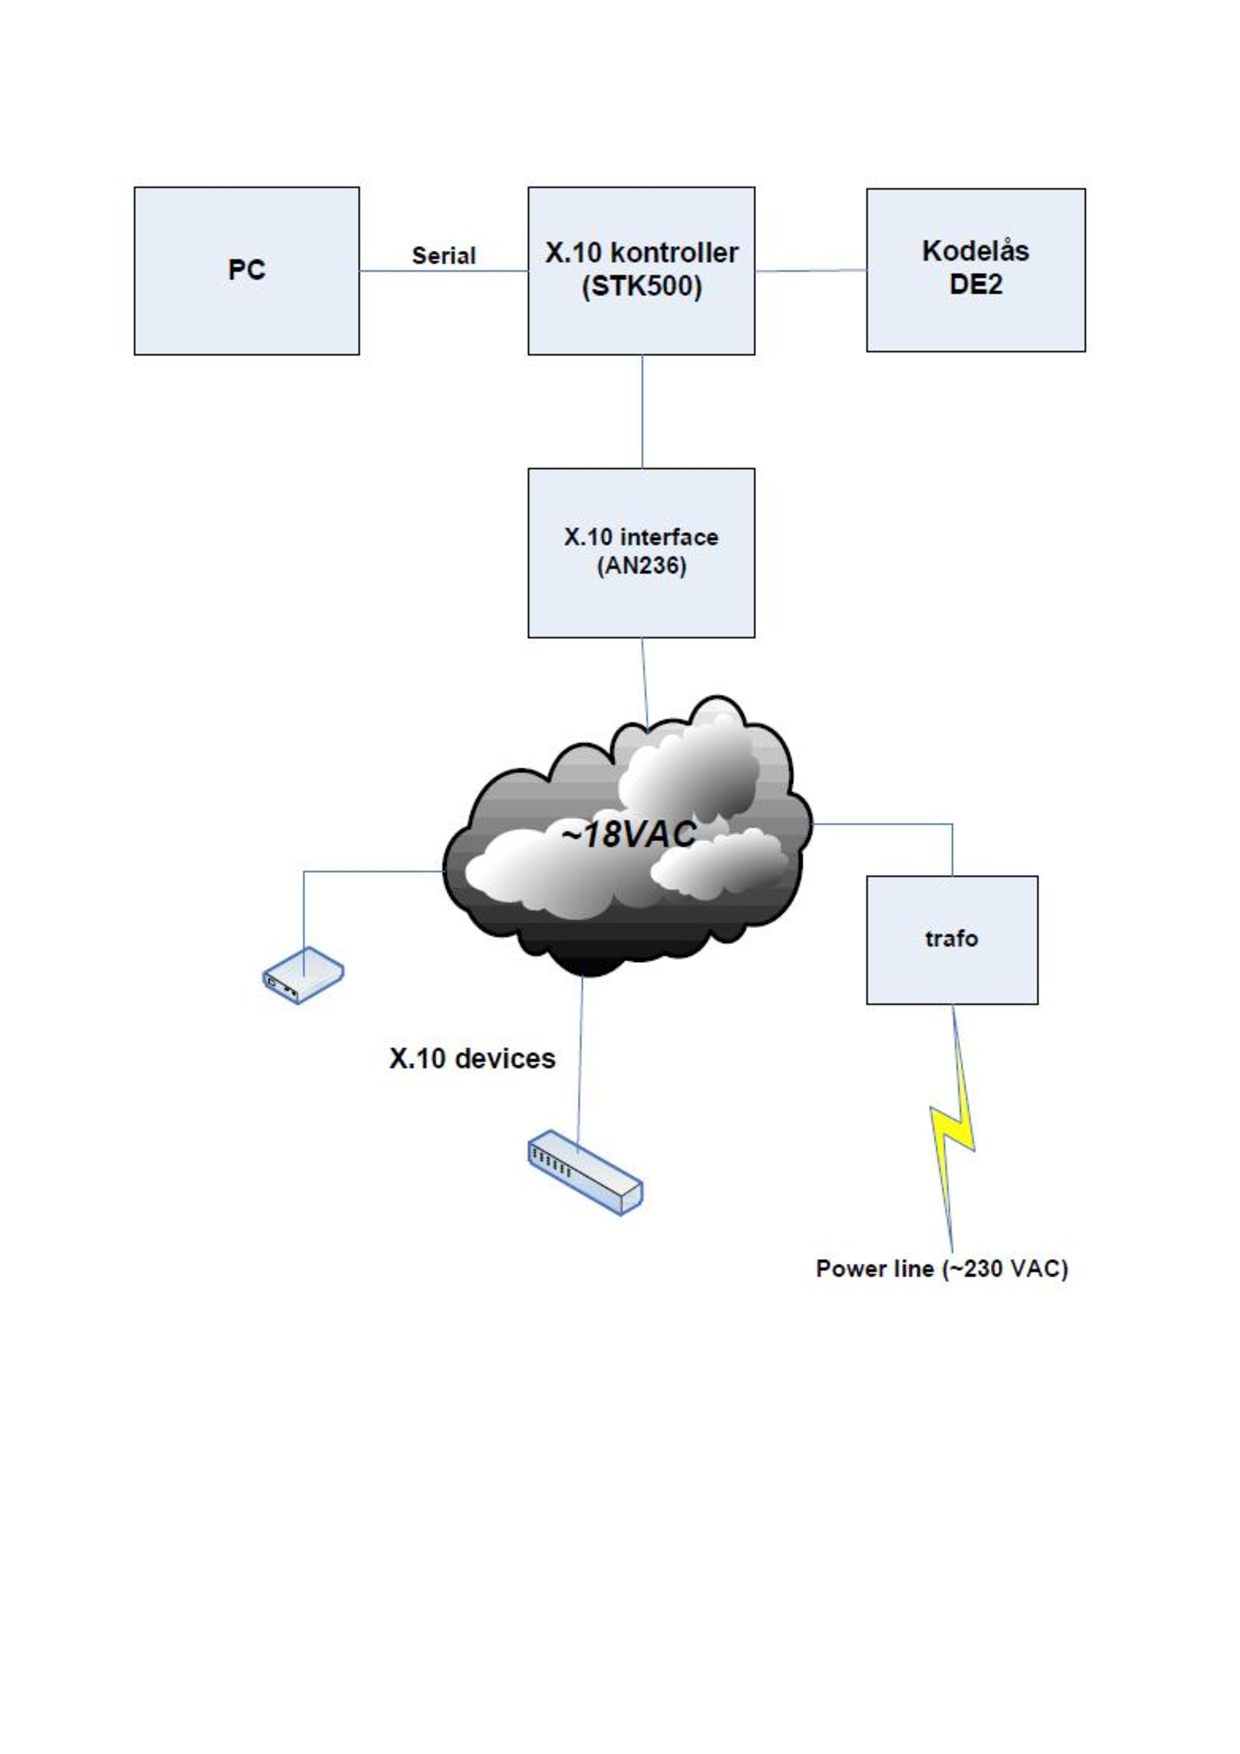
\includegraphics[width={\textwidth-2cm}, trim=0 220 0 50, clip=true] {Opgaveformulering/HW_setup.pdf}
\caption{Home Security System - HW setup \cite[s. 2]{lib:Projektoplaeg}}
\end{figure}

\clearpage
\chapter{Projektafgrænsning}
Der er som nævnt under opgaveformuleringen krav om at systemet skal indeholde:
\begin{itemize}
\item 1 PC som anvendes til konfiguration og styring
\item 1 STK500 kit som anvendes til central transmitter controller
\item 1 DE2-kodelås
\end{itemize}
Der er desuden krav om at X.10 protokollen \cite[s. 12]{lib:AN236} skal anvendes til kommunikation via el-nettet. 

Som det ligeledes er nævnt under opgaveformuleringen, anvendes et 18 VAC elnet i stedet for det almindelige 230 VAC elnet af sikkerhedsmæssige årsager. 

Til at starte med er det fuldstændige system beskrevet i projektdokumentationen, men af tidsmæssige årsager, er radio- og TV-delen udeladt fra og med signalbeskrivelser i Systemarkitekturen på side \pageref{P-tbl:signalbeskriv} i projektdokumentationen.
Det ville kræve en del mere arbejde at implementere kommunikationen til radio og TV fra de respektive receivere, da denne skulle foregå ved brug af infrarødt lys. 

Systemets hardware er implementeret på veroboard, hvilket betyder at accepttest af afskærmningen af elektriske komponenter ikke er gennemført. 

Kun dele af X.10 protokollen, som er relevante for opfyldelse af systemets mål, er anvendt. 
For mere detaljeret beskrivelse af den anvendte X.10 protokol henvises til afsnittet \textit{Protokol for X.10} på side \pageref{P-prot_x10} i projektdokumentationen.
\clearpage

\chapter{Systembeskrivelse}
Dette projekt omhandler som nævnt et Home Automation System, som kan anvendes til at simulere tilstedeværelse i et hjem, når ingen er hjemme. 
Dette sker ved at to lamper, et TV og en radio blandt andet tændes og slukkes på nogle foruddefinerede tidpunkter. 
Derved kan en indbrudstyv foranlediges til at tro, at nogen er hjemme, og derved kan indbrud forhindres. 

Systemet kan desuden anvendes til automatisering af brugerens hverdag, fx ved at bruge radio som vækkeur og tænde lys om morgenen, slukke alt lys om aftenen og lignende. 

Systemet er tilpasset én bestemt brugers hjem. 
Det er således ikke et universalt system, som umiddelbart kan tilpasses forskellige hjem med forskellige størrelser og behov. 
Systemet kan som nævnt styre to lamper, én radio og ét TV, herunder tænde, slukke og dimme lamper op og ned, samt anvende de mest almindelige funktioner for radio og TV (tænd, sluk, volumen, kanalvalg). 

\begin{figure} [h]
\centering
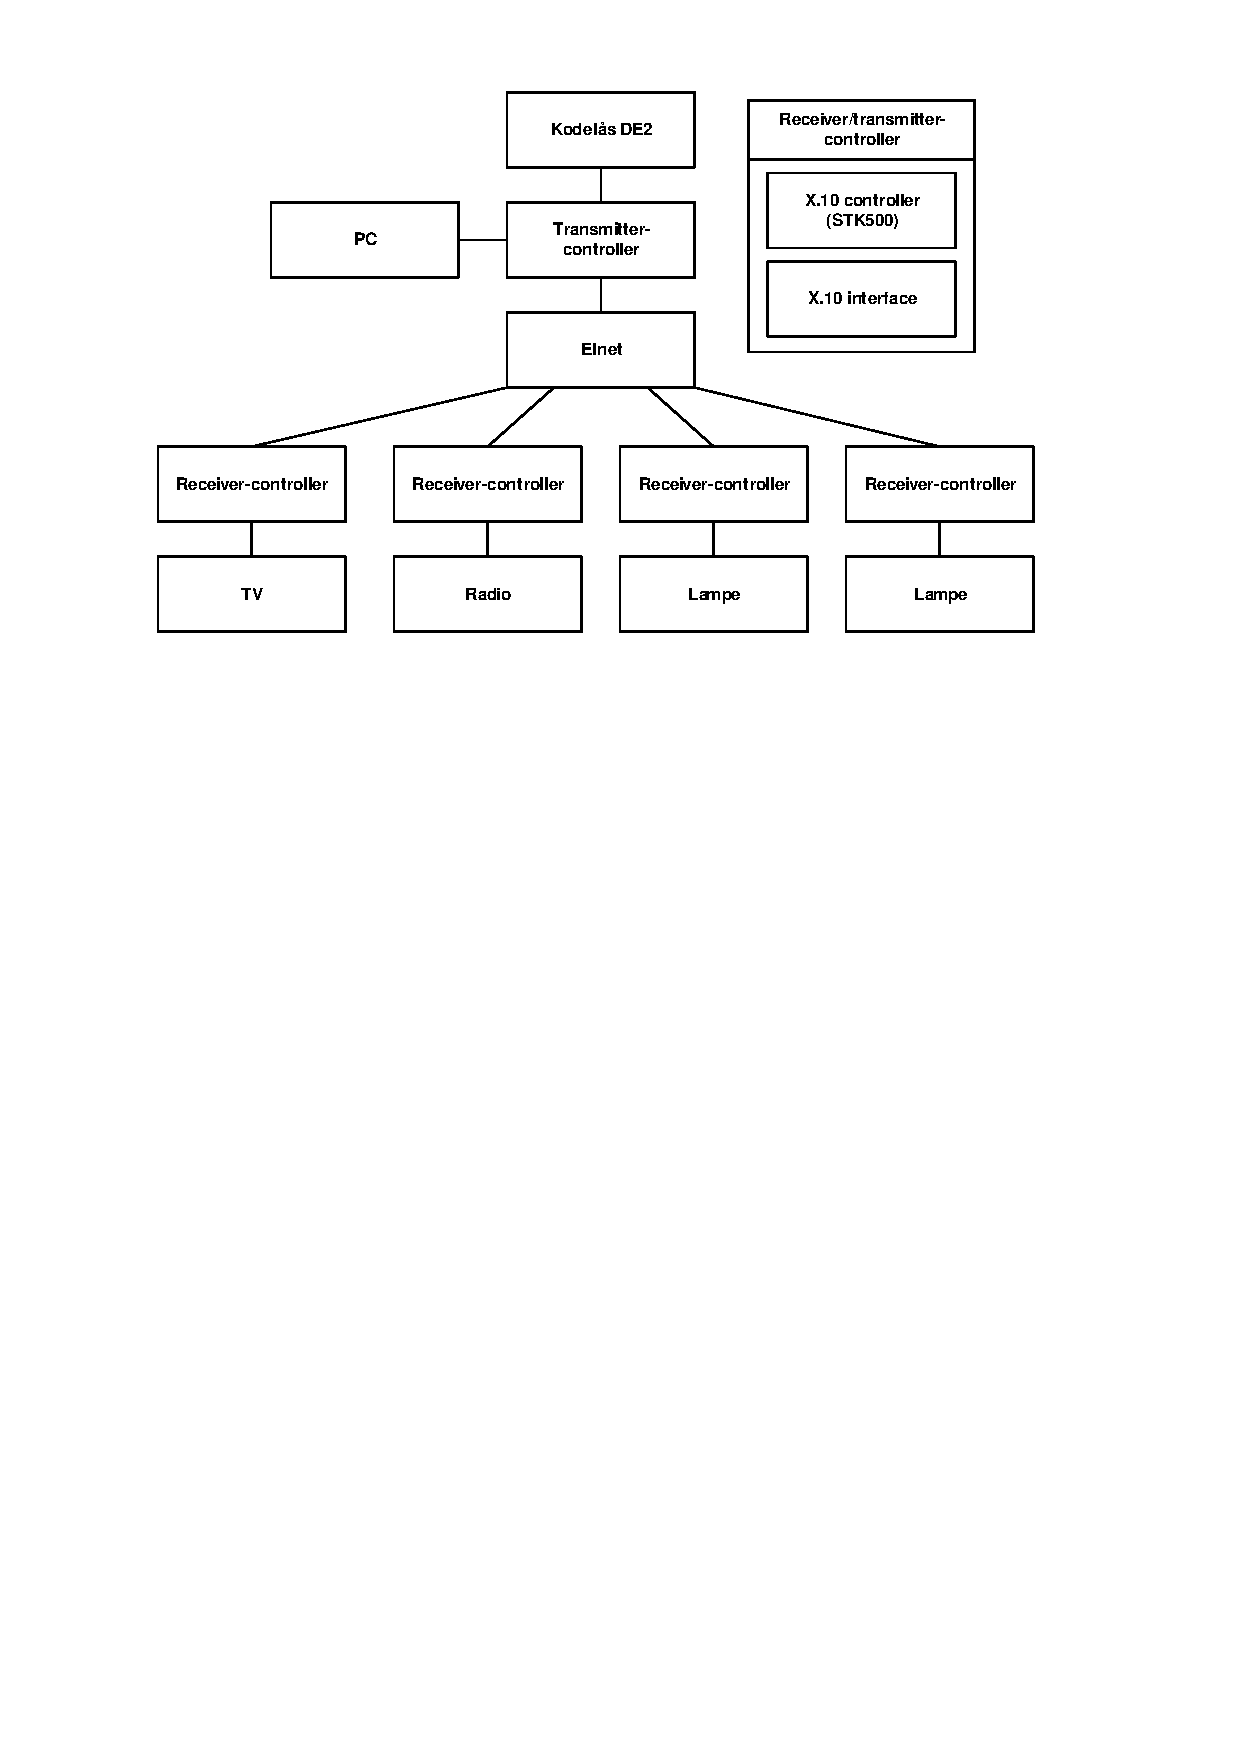
\includegraphics[scale=0.9,trim=50 535 80 40, clip=true] {../Projektdokumentation/Projektformulering/kommunikation_diagram.pdf}
\caption{Kommunikationsveje mellem enheder i systemet}
\end{figure}

Brugeren af systemet kan oprette et brugerdefineret scenarie, eller han kan vælge et af tre forudprogrammerede scenarier. 
Når et scenarie startes, simuleres tilstedeværelse i hjemmet ved at lamper, radio og TV tændes, slukkes etc. 
Et scenarie varer 24 timer og gentages indtil brugeren stopper det eller starter et andet scenarie. 
Et brugerdefineret scenarie gemmes ikke til senere brug, det eksisterer kun på transmitter controlleren så længe det afvikles. 

Der er i systembeskrivelsen lagt stor vægt på at systemet skulle være så simpelt som muligt. 
Dette er sket ud fra en tanke om at lille kompleksitet giver stor pålidelighed, samt at gruppen har valgt at fokusere på at lære så meget som muligt omkring processen i et ingeniørprojekt. 
Dette betyder selvfølgelig også en begrænset funktionalitet, men det er forsøgt at finde et fornuftigt leje, som sikrer udfyldelse af systemets mål. 
Der er således rimelig begrænset funktionalitet i systemets software, fx gemmes brugerdefinerede scenarier ikke. Hardwaren er opdelt i underdele – byggesten – hvoraf nogle genanvendes flere steder i systemet. 
Systemet indeholder kun envejskommunikation, dvs. den centrale transmitter modtager ikke informationer om en afsendt kommandos gennemførelse, hvilket kunne have givet ekstra sikkerhed for funktionaliteten. 

For yderligere information henvises til \textit{systembeskrivelsen} på side \pageref{P-Systembeskrivelse} i dokumentationen. 

\clearpage
\chapter{Krav}
\begin{figure}[h]
\centering 
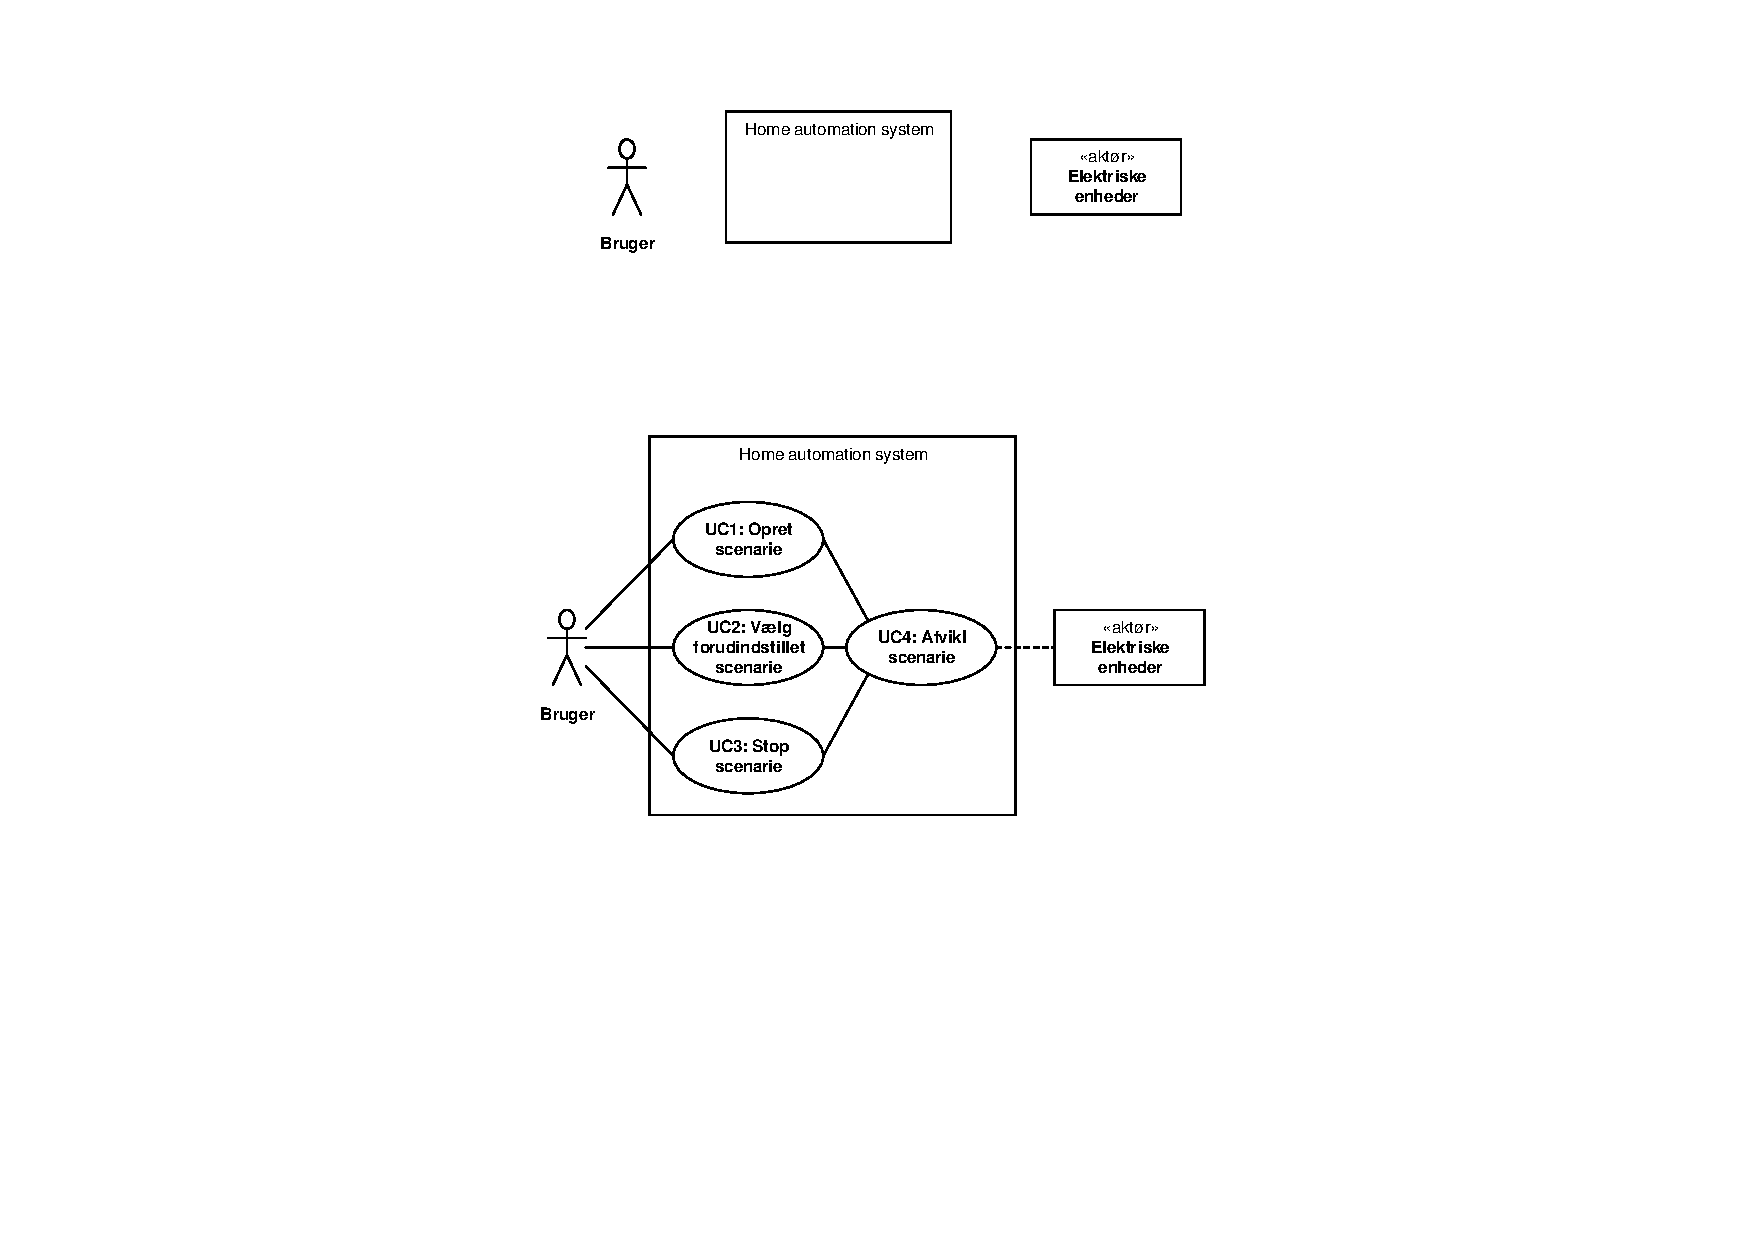
\includegraphics[width=\textwidth, trim=190 200 230 200, clip=true] {../Projektdokumentation/Kravspecifikation/actor.pdf}
\caption{Use Case diagram}
\label{UC diagram}
\end{figure}
De funktionelle krav for systemet er detaljeret beskrevet under \textit{Funktionelle krav} på side \pageref{P-FunkKrav} i dokumentationen, men Use Cases i Figur \ref{UC diagram} diagram giver et overordnet overblik. 

\begin{itemize}
\item UC1: Opret Scenarie 

Giver brugeren mulighed for at oprette et brugerdefineret scenarie, som derefter kan afvikles i systemet (UC4: Afvikl Scenarie). Et scenarie kan indeholde op til 20 aktioner, der hver især udfører en handling (tænd, sluk etc.) for en enhed (lamper, radio, TV) på et tidspunkt fastsat af brugeren. Et brugerdefineret scenarie gemmes som nævnt ikke til senere brug, men eksisterer på transmitter controlleren så længe det er under afvikling. 

\item UC2: Vælg Forudindstillet Scenarie 

Giver brugeren mulighed for at vælge et af tre forudprogrammerede scenarier. Disse tre scenarier ligger i PC-softwaren, og sendes til transmitter controlleren hver gang de skal afvikles (UC4).

\item UC3: Stop Scenarie 

Giver brugeren mulighed for at stoppe et igangværende brugerdefineret eller forudindstillet scenarie. Når brugeren vælger at stoppe et scenarie, slukkes alle tilkoblede enheder.  

\item UC4: Afvikl Scenarie 

Brugeren kan ikke interagere direkte med denne use case. Han kan initiere denne use case indirekte via UC1 eller UC2, og han kan stoppe den indirekte via UC3. 
\end{itemize}

Der er desuden formuleret en række ikke-funktionelle krav, som medvirker til sikring af systemets kvalitet og opfyldelse af projektets afgrænsninger. Disse er nærmere beskrevet i afsnittet \textit{Ikke Funktionelle Krav} på side \pageref{P-ikkeFunkKrav} i projektdokumentetionen.
\clearpage
\chapter{Projektbeskrivelse}
\section{Projektgennemførelse}
Som noget af det første udarbejdede gruppen en samarbejdsaftale \cite{lib:Samarbejdsaftale}, der fastlagde rammer for gennemførelse af projektet. 

Det er klart, at selve punkterne i aftalen har haft betydning for projektarbejdet, men også processen i at lave aftalen, var særdeles givende. 
Gruppen havde ikke arbejdet sammen som helhed før, så det var vigtigt at få afstemt forventninger til arbejdet, herunder særligt ambitionsniveauet for projektet. 


Der var således fra starten enighed om at gruppens prioriterede ambitioner var:

\begin{enumerate}
\item At lære mest muligt.
\item Lave en god rapport og dokumentation.
\item Lave et komplekst fungerende system.
\end{enumerate}

Der er undervejs i arbejdet – særligt i de tidlige faser – lagt stor vægt på at arbejde så meget sammen som muligt, for at optimere fælles læring og vidensdeling. 
Meget store dele af dokumentationen er derfor skrevet i fællesskab. 
Det har medvirket til et bedre resultat, men det har også betydet, at nogle faser har taget længere tid, end hvis opgaver var blevet fordelt mellem gruppemedlemmer og efterfølgende samlet. 

Samarbejdsaftalen indeholder også rammer for gruppearbejdet, såfremt et eller flere gruppemedlemmer ikke levede op til aftalen. 
Dette har ikke været på tale, efter rammerne var fastlagt. 
Alle i gruppen har været særdeles engagerede, hvilket selvfølgelig har været meget positivt, men det har også betydet, at gruppen nogle gange har skullet bruge en del ressourcer på at finde kompromis mellem mange inputs og meninger om store eller små ting. 

Samarbejdsaftalen placerede desuden en række ansvarsområder til enkelte gruppemedlemmer. 
Der er senere i forløbet blevet fordelt flere områder:
\begin{itemize}
\item Koordinator

Morten har haft dette ansvarsområde, og dermed ansvar for mødeindkaldelser, mødereferater, føring af overordnet log, opdatering af fælles kalender, opdatering af tidsplan mm. 

\item Ordstyrer

Dette område har gået på skift mellem gruppemedlemmerne for 2 uger af gangen. 
Det har primært indebåret ordstyring under gruppemøder og fælles arbejdsmøder.

\item Dropbox ansvarlig

Kristian T. har haft dette ansvarsområde og dermed ansvar for vores fælles filstruktur til deling af dokumenter.

\item Apache Subversion

David har haft ansvar for dette værktøj, som har været anvendt til versionsstyring og deling af kildekode. 

\item Latex ansvarlig

Kristian S. og Kristian T. har haft dette område. 
Gruppen valgte på et tidligt tidspunkt at rapport og dokumentation skulle skrives med dette værktøj. 
Ansvarsområdet har indebåret afholdelse af en lektion for øvrige gruppemedlemmer og løbende hjælp til brug af værktøjet. 

\item Scrum ansvarlig

David har fungeret som Scrum ansvarlig i de faser hvor Scrum er blevet anvendt. 

\item HW ansvarlig

Morten har under design og implementering af hardware fungeret som koordinator for dette.

\item SW ansvarlig

Kasper har under design og implementering af software fungeret som koordinator for dette. 
\end{itemize}


Som tidligere nævnt har der under projektarbejdet været lagt vægt på, at hele gruppen arbejdede sammen så meget som muligt, men under design og implementeringsfaserne blev gruppen delt op i undergrupper. 
Det skete i første omgang ved at Kasper, David, Kristian T. og Kristian S. udarbejdede SW design, mens Morten, Henrik, Lasse og Philip lavede HW design. 
Under implementeringsfasen blev Morten og Kasper i deres respektive grupper, og fungerede som tovholdere for disse, mens de øvrige medlemmer i projektgruppen havde mulighed for at arbejde med implementering inden for begge områder. 

Kommunikationen internt i gruppen har foregået via en fælles Facebook gruppe og ugentlige arbejdsmøder, hvilket har fungeret godt.

Den fælles kalender på Ingeniørhøjskolens Campusnet har været anvendt til at holde styr på vejledermøder, arbejdsmøder og øvrige aftaler.
 
I starten af forløbet blev der udarbejdet en overordnet tidsplan \cite{lib:Tidsplan}, ud fra en skabelon i projektoplægget \cite{lib:Projektoplaeg} med deadlines for review mm.
Gruppens egen tidsplan blev fastlagt således, at projektarbejdet så vidt som muligt var en uge foran. 
Dette skete på baggrund af, at der så ville være tid til uforudset arbejde og skrivning af rapport. 
Det er med lidt svingende udfordring lykkes at holde denne tidsplan, hvilket har givet projektgruppen ekstra god tid, særligt i de sidste faser.

Undervejs i projektarbejdet har der været afholdt to reviews \cite{lib:Review1} \cite{lib:Review2}, hvor projektarbejdet er blevet gennemset og kommenteret af en anden gruppe og vice versa. 
Det har naturligvis betydet ekstra arbejde at skulle gennemse en anden gruppes arbejde, men kommentarene fra en anden projektgruppe og deres vejleder, samt fra denne projektgruppes egen vejleder, har været givende for det endelige resultat. 

\section{Metoder}

\subsection{SysML}
SysML har givet et bedre overblik over projektet, da systemet har kunnet deles op i blokke, og det herefter var muligt at arbejde med de individuelle blokke. Ud fra disse enkelte blokke, var opdelingen af parts og ports nemt. 
BDD-diagrammer har givet overblik over kompostion af blokkene via relationer, som er specificeret i diagrammet.
IBD-diagrammer har givet mulighed for at holde styr på signaler, og kommunikationsveje mellem de forskellige blokke. Signalerne, der går imellem blokkene, gav mulighed for at lave detaljerede grænseflader på systemets elementer, og i såfald hvilken type, da det vides, om der skal forekomme kommunikation mellem disse elementer. 
Use Cases har givet mulighed for at designe det ønskede scenarie, og tage højde for de faldgrupper, der kan opstå undervejs i scenariet. Use Cases er blevet anvendt til at fremstille sekvensdiagrammer, så de stemmer overens med udførelsen af de enkelte steps i use casen.

\subsection{Scrum}
Scrum er blevet brugt til uddeling og adminstration af opgaver under projektet. Standard scrum-roller blev ikke brugt, men i stedet var der et fælles ansvar for at få lagt opgaver ind på scrum-boardet. Da der ikke var et fast grupperum til projektarbejdet, var det ikke muligt at bruge et klassisk scrum-board, og der blev derfor anvendt en webbaseret løsning i stedet  \cite{lib:Axosoft}. Der blev brugt en form for daglige Scrummøder. Alle medlemmer kunne hver især kort fremlægge, hvad de  havde lavet, og hvad planen for resten af dagen var. De mange opdateringer på fremskridtet med arbejdet, bidrog til at der var en konstant ide om, hvor langt projektgruppen var nået i den nuværende fase. Det startede ud med, at Scrum blev testet i Softwaregruppen under designfasen, da der var mange små opgaver, som skulle løses, hvilket gjorde det nemmere at holde styr på hver opgaves status, så intet blev glemt. Efter design-fasen blev alle medlemmer af gruppen introduceret til brugen af Scrum, da der i gruppen var interesse for at arbejde med både software og hardware.
På grund af relativ få opgaver i hardware-gruppen, synes flere at scrum-boardet ikke bidrog til overblik i udviklingen. Til udvikling af software har scrum-boardet været godt til at danne overblik over de mange mindre opgaver som systemet bestod af.

\subsection{V-model og ASE-model}
I projektet har V-modellen\cite{lib:Projektoplaeg} været anvendt indtil modul-designet, hvor der blev skiftet over til at bruge ASE-modellen. 
ASE-modellen var blevet brugt i fuld form i arbejdsfordelingen. Arbejdet blev delt op i software og hardware, under design og implementering. Det har gjort arbejdet mere effektivt, da det har givet den enkelte mulighed for mere fordybelse til at arbejde med et specifikt område. Efter de forskellige moduler har været igennem modultest, begyndte integrationstesten samlet, hvor hardware og software skulle samles.

\subsection{Versions-styring}
Versioner på dokumentations-dokumenter er blevet opdateret løbende med kommentarer fra vejleder og reviews. Væsentlige ændringer i design og dokumentation har givet anledning til versions-ændring, hvilket hjælper med at holde styr hvilke ændringer projektet har gennemgået.

\subsection{Review}
De reviews\cite{lib:Review1}\cite{lib:Review2}, der var modtaget, hjalp til med at opdage fejl og mangler i dokumentationen, som efterfølgende blev rettet på et arbejdsmøde. 
De reviews, som skulle fremstilles, har givet mere inspiration til gruppens eget projekt, og givet kompetencer indenfor rettelse af tekniske dokumenter. At påpege fejl og mangler, i stedet for at komme med forslag til forbedring, gjorde reviewet mere objektivt til andres arbejde. Når der modtages review, holdes det på et neutralt plan, og der forsøges ikke at forsvare den skrevne dokumentation, men istedet skal den modtagende gruppe koncentrere sig om de modtagne kommentarer. Kommentarene kunne diskuteres på et efterfølgende møde, og de vigtige mangler og fejl kunne rettes i dokumentationen.


\section{Fildeling}

\subsection{Dropbox}

Gennem projektet har Dropbox været den primære fildelings service til at holde styr på alt undtaget kildekode. Beslutningen skyldes at alle medlemmer i gruppen har erfaring med Dropbox, og det var nemt at sætte op. Dropbox indeholdte mødereferater, tidsplan, coaching, diagrammer samt andre bilag. 
Mappe-strukturen var en stor hjælp angående indeksering af tex-filer, og generelt har brugen af Dropbox gennem forløbet været uproblematisk. Desuden har Dropbox's restorefunktion som har reddet rapporten, da den blev fejlagtigt slettet.

\subsection{SVN}

Til deling af kildekode var overvejelserne mellem Git og SVN. Git var interessant, da flere virksomheder bruger dette, og det vil give noget relevant erfaring. SVN blev dog valgt til deling af kildekode, siden et gruppemedlem havde et SVN repository oppe på \url{riouxsvn.com}, samt ISE faget gav undervising i brugen af SVN. Sidst skal det fremhæves, at den klient vi valgte at bruge, TortoiseSVN\cite{lib:Tortoise}, har meget simpel tilgang til de mest væsentlige kommandoer, \texttt{update} og \texttt{commit}, mens git umidelbart havde en mere kompliceret tilgang. Så simplicitet var valgt over funktionalitet.

SVN blev kraftigt brugt gennem software implementeringsfasen, og endte med 88 revisioner. I starten var der lidt problemer med committing, dog blev dette løst hurtigt, efter folk blev bekendte med tjenesten.
   
\documentclass[a4paper,11pt,oneside,article]{memoir}
\renewcommand{\baselinestretch}{1.05}
\usepackage{amsmath,amsthm,verbatim,amssymb,amsfonts,amscd, graphicx}
\usepackage{graphics}
\usepackage[utf8]{inputenc}
\usepackage[danish]{babel}
\topmargin0.0cm
\headheight0.0cm
\headsep0.0cm
\oddsidemargin0.0cm
\textheight23.0cm
\textwidth16.5cm
\footskip1.0cm
\theoremstyle{plain}
\newtheorem{theorem}{Theorem}
\newtheorem{corollary}{Corollary}
\newtheorem{lemma}{Lemma}
\newtheorem{proposition}{Proposition}
\newtheorem*{surfacecor}{Corollary 1}
\newtheorem{conjecture}{Conjecture} 
\newtheorem{question}{Question} 
\theoremstyle{definition}
\newtheorem{definition}{Definition}

\begin{document}

\frontmatter

\title{Latex}

\author{Kristian}

\maketitle

\clearpage

\mainmatter

\chapter{Brug af LaTex}

\begin{enumerate}

 \item Åben Template.tex med texmaker.
 
 \item Tryk F1, og texmaker begynder en "quick build". Du burde nu se et vindue med din pdf, ellers tryk F1 igen.
 
 \item Over i din tex fil, vil du se \textbackslash title \{ Latex \} . Erstat "Latex" med "Mit første latex dokument" og tryk F1.
 
 \item Du kan kan gøre det samme med \textbackslash author \{ mit navn \} og tryk F1 igen. 
 
\end{enumerate}

(Du behøver ikke trykke F1 efter hver lille ændring) 


\chapter{Layout}

\section{Sections og subsections}

Latex består af kapitler og sektioner (og derunder undersektioner og underundersektioner). Formatet er det samme, $\backslash chapter \{ Something \}$, Hvor "Something" er navnet på din afsnit. Prøv at indsætte $\backslash chapter \{ Something \}$ under $ \backslash maketitle$ i din tex dokument og tryk F1. \\
\\
Du kan også lave afsnit med $\backslash section \{ Something else \}$. Prøv at indsætte 
$\backslash section \{ Something else \}$ under $\backslash chapter \{ Something \}$ i din tex dokument og tryk F1. \\
\\
Under $\backslash section \{ Something else \}$ kan du skrive din tekst til afsnitet. Prøv at skrive en lille tekst, og derefter compile med F1.\\
\\
Du kan ligeledes lave underafsnit med $\backslash subsection \{Something \}$ og underunder afsnit med $\backslash subsubsection \{Something \}$. Du behøver ikke lave afsnit eller underafsnit for at skrive brød tekst, men det ser bedre ud.

\section{Newpage og newline}

Hvis du gerne vil starte på en ny side, så skriv $\backslash newpage$.

Ønsker du at lave en ny side, hvor floats (billeder, tabeller etc.) ikke følger med fra de forrige sider, bruger du $\backslash clearpage$. \\

$\backslash \backslash$ efter en linie tekst giver en newline.

\newpage

\chapter{Billeder/tabeller}

\section{Import billeder}

\begin{enumerate}

	\item Find et billede, du gerne vil indsætte, og læg det i samme mappe som din tex fil.

	\item Under din lille tekst fra forrige øvelse indsæt $\backslash includegraphics[scale=1]{pic.png}$
	
	\item Erstat pic.png med navnet på dit billede (husk at tilføre fil- typen på dit billede som vist i 		  eksemplet) 
	
	\item Scale sætter hvor stort billedet skal være, Så scale=0.5 sætter billedet til halv størrelse.

\end{enumerate}


\section{Tabel}

Skriv en sandhedstabel for en AND-gate. \\
\\
Brug http://en.wikibooks.org/wiki/LaTeX til at finde ud af hvordan tabeller laves.

\chapter{Matematik}

Matematiske formler kan skrives på flere forskellige måder. \$ math formel \$ giver et "matematikfelt" in-line, dvs det kan skrives i brødteksten. $\backslash begin \{ displaymath \}$ giver et matematikfelt på sin egen linie og i midten. $\backslash begin \{ equation \}$ gør ca det samme som $displaymath$, men giver linien et nummer, som man kan sætte en label på med $\backslash label \{something \}$ og derefter referere til med $\backslash ref \{something \}$. Indskriv \\
 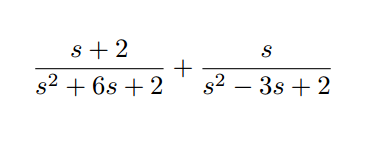
\includegraphics[scale=1]{../lektion/math.png} \\
i latex vha. http://en.wikibooks.org/wiki/LaTeX/Mathematics.


\end{document}
\section{Specifikation og Analyse}
Denne sektion omhandler hvordan der er blevet analyseret og specificeret i projektets overordnede problemløsninger af de opstillede problemer under projektoplæget. 
Dette vil omhandle bearbejdelsen og tankerne bag kravspecifikationen (side \pageref{P-chap:kravspec} i projektdokumentation).

For at specificere problemet der skulle løses, blev der diskuteret mellem projektets medlemmer, om hvad der er det primære formål med dette projekt var. 
Inden andet blev foretaget, blev de forskellige krav, der blev stillet fra projektoplæget, undersøgt. 
Der blev taget en beslutning om funktionaliteten af det endelige system, således at det passede til formålet beskrevet under projektoplæget. 
Projektgruppen fandt individuelle løsninger på det primære problem og præsenterede disse løsninger for de øvrige medlemmer. 
Dette resulterede i at gruppen valgte at Home Automtion Systemet skulle have tilkoblet to lamper, et TV og en radio og at det skulle tilgås via en PC og ellers køre fra en microcontroller, som kommunikerede via X.10\cite{lib:AN236} til øvrige microcontrollere på et $18V AC$ netværk. 
Den oprindelige tanke var at TV og Radio skulle styres vha infrarød kommunikation fra deres respektive modtagere, men gruppen fravalgte dette inden design-fasen, for at fokusere på det vigtige aspekter i projektet, nemlig at få protokollen og kommunikation via X.10 til at fungere.
Dette blev herefter dokumenteret i form af \textit{Systembeskrivelse} på s. \pageref{P-Systembeskrivelse} og \textit{Aktør-kontekst diagram} på s. \pageref{P-fig:actor} under Kravspecifikation i projektdokumentationen.

Herefter blev et use case diagram, samt use case beskrivelse, for de primære hovedforløb af systemets ønskede funktionalitet, konstrueret således, at der ikke kunne opstå tvivl, i det ønskede systems funktionalitet og formål samt for at skabe overskuelighed af systemet. 
Ud fra formål, funktionalitet og use cases blev der opstillet krav til det endelige system. 
Disse krav blev inddelt i funktionelle og ikke funktionelle krav (s. \pageref{P-FunkKrav} i Projektdokumentationen) således, at de valgte arbejdsmodeller blev fulgt, og det var muligt at opstille en endelig kravspecifikation under processen. 
Dette endte ud i at en accepttest (s. \pageref{P-chap:acceptt} i dokumentationen) var mulig at udarbejde, dermed blev V-modellen fulgt.
\clearpage

\section{SystemArkitektur}

\subsection{SysML} 

\begin{figure}[h]
	\centering \resizebox{\textwidth}{!}{
	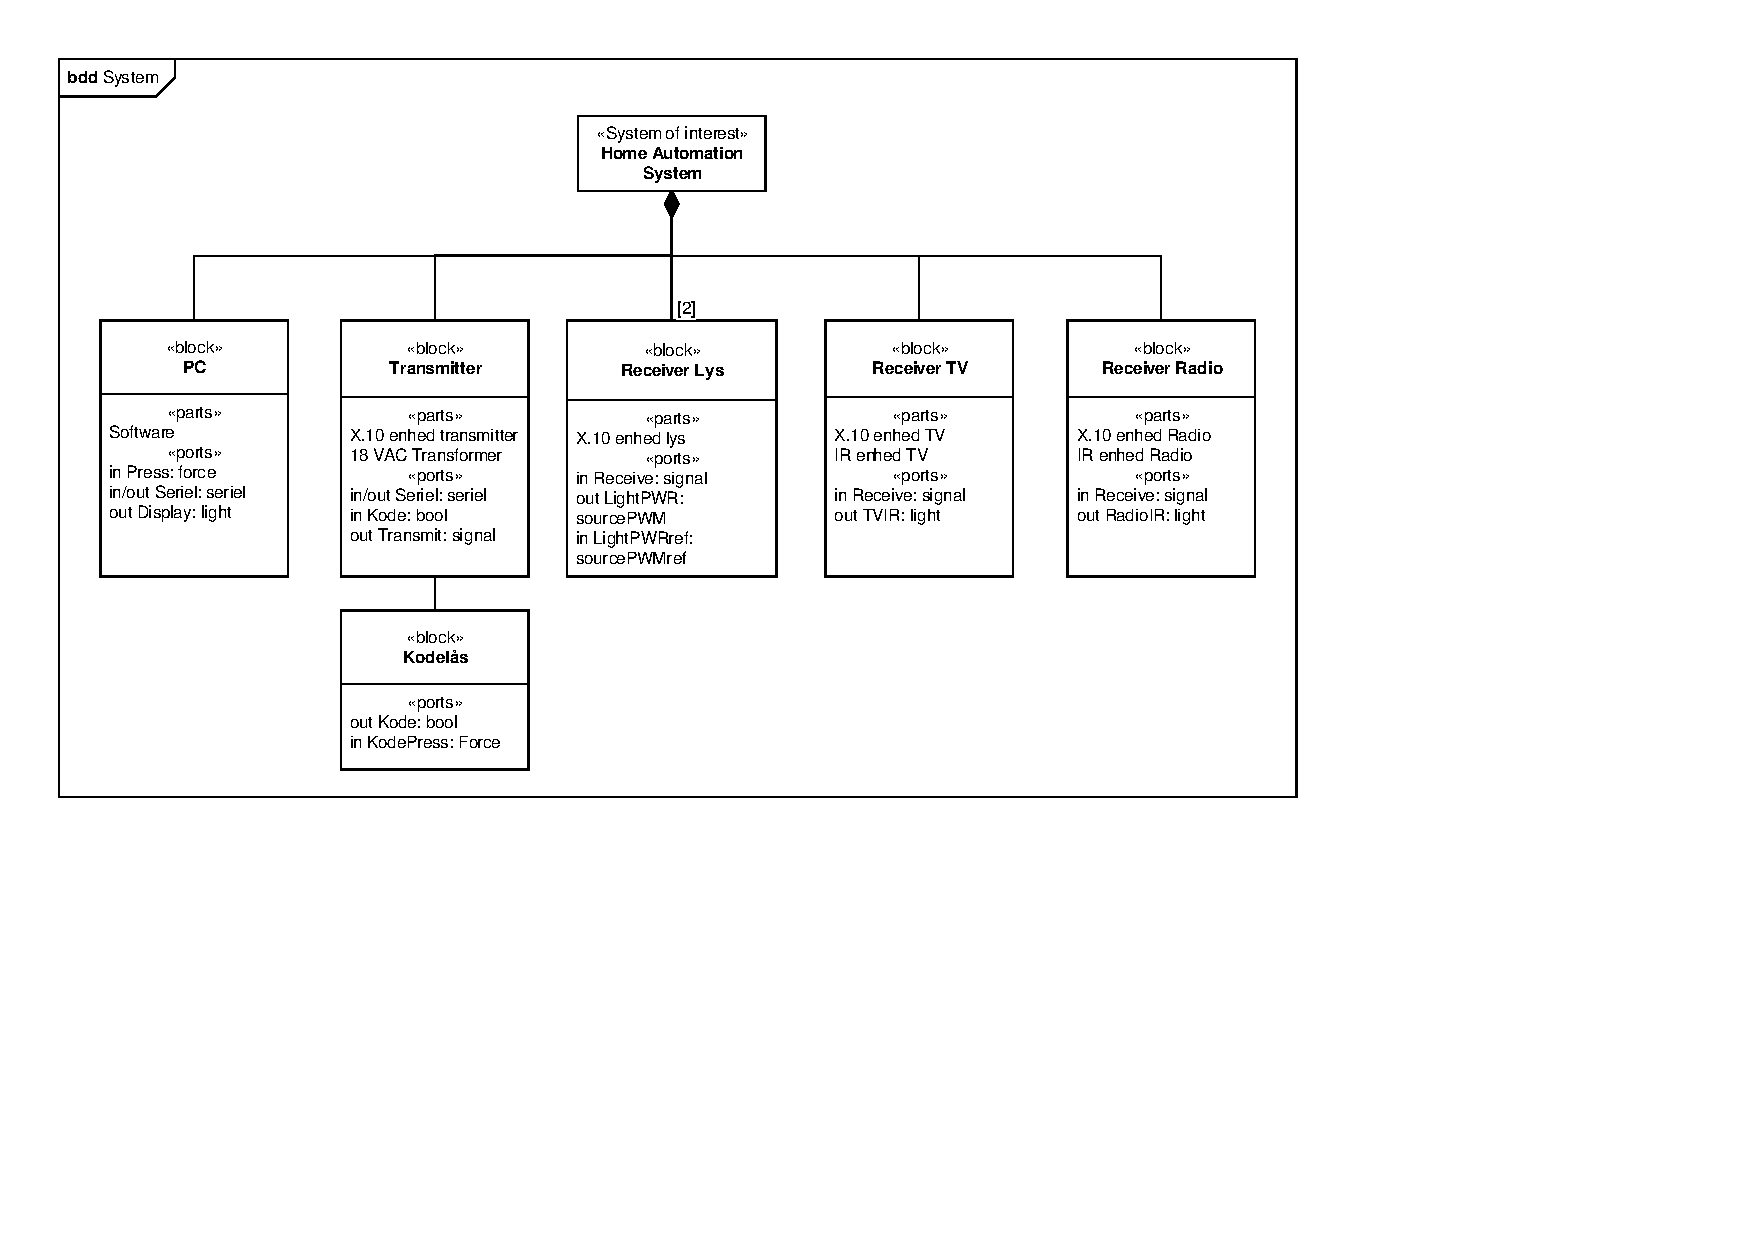
\includegraphics[scale=1,trim=28 210 219 25, clip=true]{Projektbeskrivelse/Systemarkitektur/diagrammer/BDD_System.pdf}}
	\caption{BDD diagram for systemet}
\end{figure}

I systemarkitekturen blev der lavet blokke for alle elementer, og det blev forklaret hvad disse enkelte blokke består af. Dette hjalp til at give et bedre overblik over systemet. BDD'er og IBD'er er anvendt fra ISE undervisningen. BDD'erne er brugt til at beskrive, hvilke komponenter systemet består af, og som det ses på overståene BDD-diagram, er der lavet en blok for hver del: PC, Transmitter, Receiver lys, Receiver tv og Receiver radio.

IBD'erne er brugt til at vise signaltyper mellem blokkene, derudover beskriver de også systemets forbindelser. Forbindelserne har i hver sin ende nogle flowports, disse bruges til at synliggøre signalets retning og sammenhæng med andre flowporte. For hvert enkelt blok er udarbejdet en IBD, så det under design fasen er nemt at se sammenkoblingen mellem de enkelte elementer.

På baggrund af IBD'erne blev der udarbejdet en signalbeskrivelse, som ved hjælp af diverse datablade sikrer at systemet overholder alle elementernes tolerancer, så der ikke bliver ødelagt noget.

\subsection{Applikationsmodel}

Applikationsmodellen var valgt primært for softwareudviklernes skyld, da det gav en systematisk måde at opbygge softwareklasser på. Ved at se Use Cases igennem, blev der fundet konceptuelle klasser, som igen blev brugt til at bestemme hvilke kllasser, der gav mening at oprette. Efter klasserne var valgt, blev de klassificeret yderligere i hhv. boundary-, domain- og controllerklasser. Disse bruges til at holde styr på, i hvilke klasser funktionaliteten skal være.
Herefter blev der lavet sekvensdiagrammer, hvori der tages udgangspunkt i en Use Case, så metoder kan findes ud fra, hvad der skal ske for at den pågældende Use Case bliver opfyldt.

\clearpage
\section{Udviklingsværktøjer}
Under denne sektion vil der blive gennemgået de forskellige udviklingsværktøjer som hovedsageligt er blevet anvendt under dette projekts design-, implementerings- og integrationsproces.

\subsection{Multisim}
Gruppen har valgt multisim til design og simulering af hardware. Styrkerne ved multisim er at skabe et overblik og muligheden for at simulere forskellige hardware moduler, med de ønskede komponenter, fra et rigt bibliotek. Svaghederne ved multisim er, at det nogle gange kan være svært at simulere et kredsløb korrekt samt i værste tilfælde, at multisim ikke har mulighed for at simulere en hardware komponent.\\
I dette projekt er multisim anvendt under design og implementeringsprocessen for hardware.

\subsection{Visual Studio 2013}
Dette program er et redskab til kodning og debugging af kildekode under implementering af software.\\
I dette projekt er Visual Studio anvendt under implementerings- og integrationsprocessen for kodning af PC softwaremoduler, i C++.
Visual Studio er valgt pga. det er brugt i undervisningen.

\subsection{Atmel Studio}
Atmel studio er en forgrening af Visual Studio 2010. Programmet er anvendt til kodning og debugging af microcontrollere under implementering af software. Det har senere under forløbet vist sig at det har vakt mindre problemer at kode microcontrollerne med dette værktøj, da det under software design blev bestemt at kode i C++. Atmel Studio har en stærk compiler til C programmering, men den er ikke lige så stærk til C++, og endte med at give nogle mindre problemer under software implementeringen.

I dette projekt er Atmel Studio anvendt under implementerings- og integrationsprocessen for kodning af microcontoller software moduler, i C++. Under arbejdet med microcontrollere blev der gjort erfaringer (se s. \pageref{P-sec:micro} i projektdokumentationen). %TODO Indsæt reference til dokumentation afsnit impl.
\newpage
\section{Hardware Design og Implementering}
I det følgende afsnit beskrives hardware design- og implementeringsprocessen. Herunder hvilke løsninger der er valgt og evt. hvilke beslutninger, der ligger til grund herfor. Designet tager udgangspunkt i den forudgående systemarkitektur.\\

For mere detaljeret beskrivelse henvises til projektdokumentationen side \pageref{P-chap:HardwareDesign} for hardware design og side \pageref{P-chap:Hardwareimplementering} for hardware implementering.

\subsection{Overordnede overvejelser}
Som udgangspunkt for designet er den udleverende applikations-note AN236\cite{lib:AN236} anvendt. Det er dog ikke kun løsninger fra dette dokument, der er anvendt i systemet. Figur \ref{fig:HWBDD} giver et overblik over hvilke hardware-elementer, der indgår i systemet.

\begin{figure}[h]
	\centering
	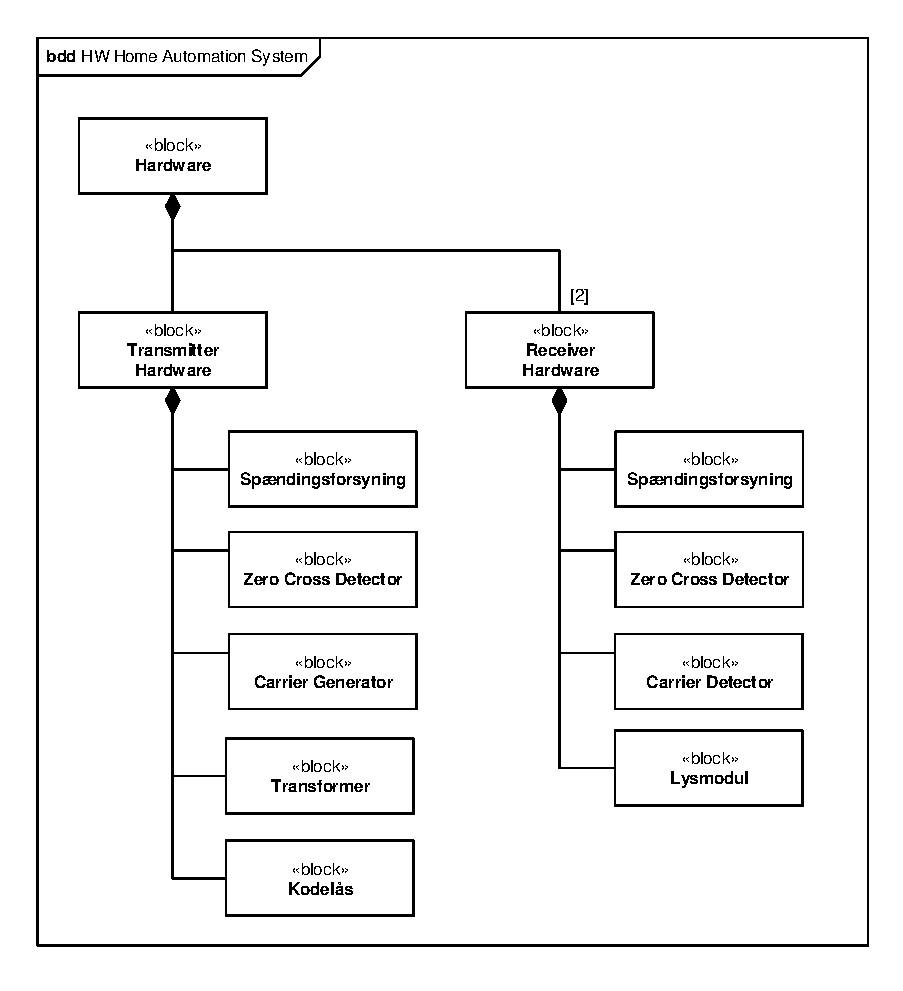
\includegraphics[scale=0.8, trim=10 10 10 10, clip=true]{../Projektdokumentation/HardwareDesign/Diagrammer/BDD_HW.pdf}
	\caption{BDD-diagram over hardware}
	\label{fig:HWBDD}
\end{figure}



Systemets hardware er opdelt i en transmitter- og to receiverdele. De underblokke, der optræder flere steder i systemet, er ens, og kan derfor betragtes som "byggeklodser", der hver har deres meget specifikke funktionalitet.Fordelen ved at opdele i byggeklodser, skal optræde flere steder i designet og derved undgås dobbeltarbejde. Hver underblok er kun beskrevet en gang. 

\subsection{Underblokke}

\subsubsection{Transformer}
Transformeren transformerer $230VAC$ til $18V AC$, og simulerer derved et almindeligt $230V$ el-net, der er sikkerhedsmæssigt forsvarligt at arbejde med.

\subsubsection{Spændingsforsyning}
Spændingsforsyningen anvendes i både transmitter- og de to receiver-blokke, hvor den genenerer ($12V$ og GND) til hhv. $+5V$ og $-5V$.\\

Oprindeligt blev spændingsforsyningen designet således, at den kun leverede $+5V$, men det blev erfaret under implementeringen, at bl.a. Zerocross Detektoren havde brug for $-5V$.\\

Der anvendes en fastspændingsregulator($LM7805$)\cite{lib:LM7805} og en spændings-inverter($ICL7660$)\cite{lib:IC7660}, der begge er opsat jf. standardapplikationen i deres respektive datablade. Kredsløbets færdige design kan ses på Figur \ref{fig:Stromforsyning}.

\begin{figure}[h]
	\centering
	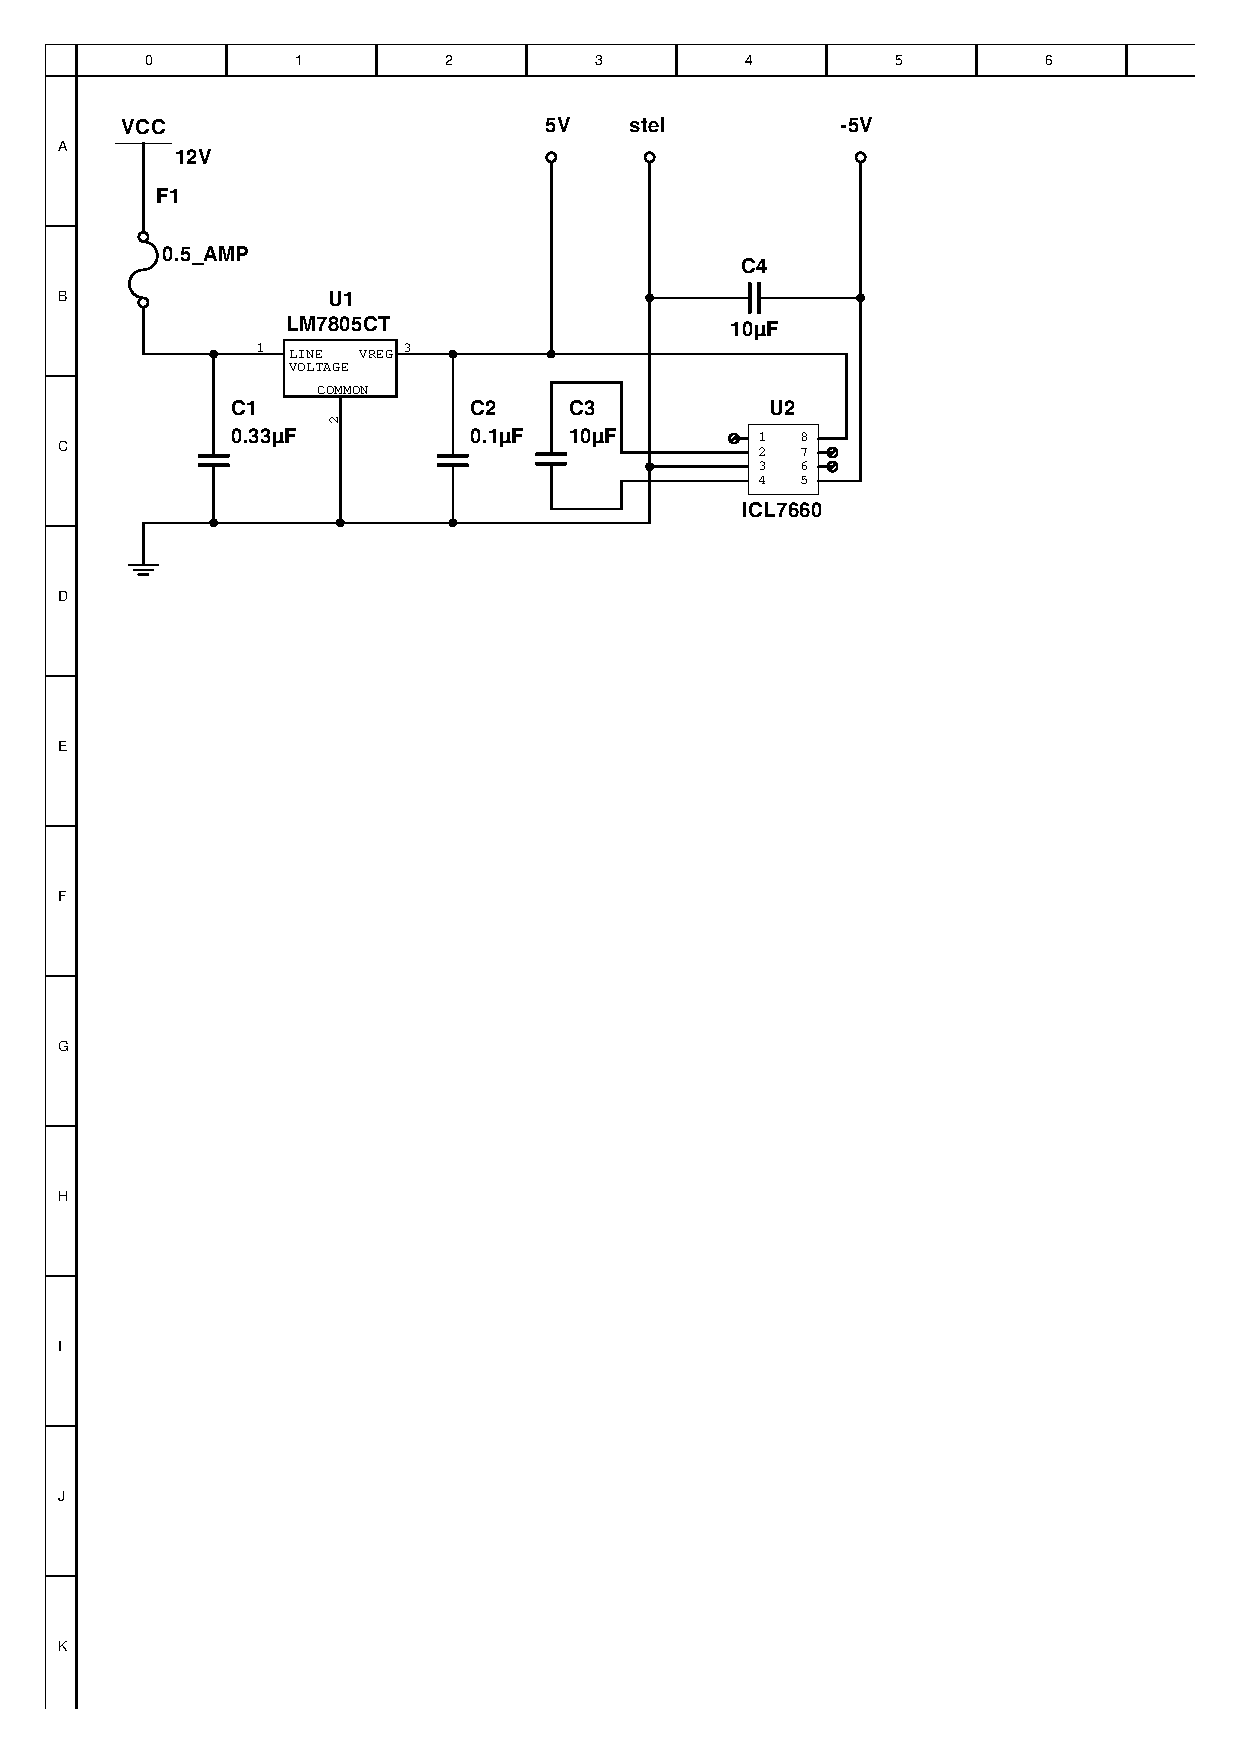
\includegraphics[scale=1,trim=50 555 150 50, clip=true]{../Projektdokumentation/HardwareDesign/Diagrammer/Stroemforsyning.pdf}
	\caption{Spændingsforsyning}
	\label{fig:Stromforsyning}
\end{figure}

En modultest af spændingsforsyningen viser at der leveres hhv. $+5.0V$ og $-5.0V$ på de respektive udgange.

\subsubsection{Kodelås}
Kodelåsen har til formål at forhindre adgang til systemet, såfremt der ikke er indtastet tre korrekte koder på DE-2 boardet, hvor kodelåsen er implementeret. Hvis der indtastes en forkert kode tre gange, vil kodelåsen låse for adgang til systemet permanent. Selve komponenten er lavet under en øvelse i faget Digital System Design og funktionaliteten er derfor ikke beskrevet yderligere.\\

Modultest og integrationstest viser at kodelåsen virker efter hensigten. Desuden er der i dokumentationen på side \pageref{P-sec:Kodelaas} gjort rede for, at udgangsspændingen ved logisk HIGH på DE2 boardet, er høj nok til at STK500-kittet registrerer det som logisk HIGH.

\subsubsection{Zerocross Detector}
Zerocross detector'en har til formål at detektere, hvornår der er en nulgennemgang på $50Hz$ nettet. Altså hvornår spændingen krydser nul. Denne information anvendes til at time hvornår der skal sendes $120kHz$ ud på $50Hz$ nettet, samt hvornår der skal læses. Når der detekteres en nulgennemgang på indgangen \textit{signal}, skal kredsløbets udgang \textit{ZeroCrossDetect} toggle mellem $0V$ og $5V$. Til at løse denne opgave er der designet et kredsløb, som vist på Figur \ref{fig:ZeroCrossDetect}.

\begin{figure}[h]
	\centering
	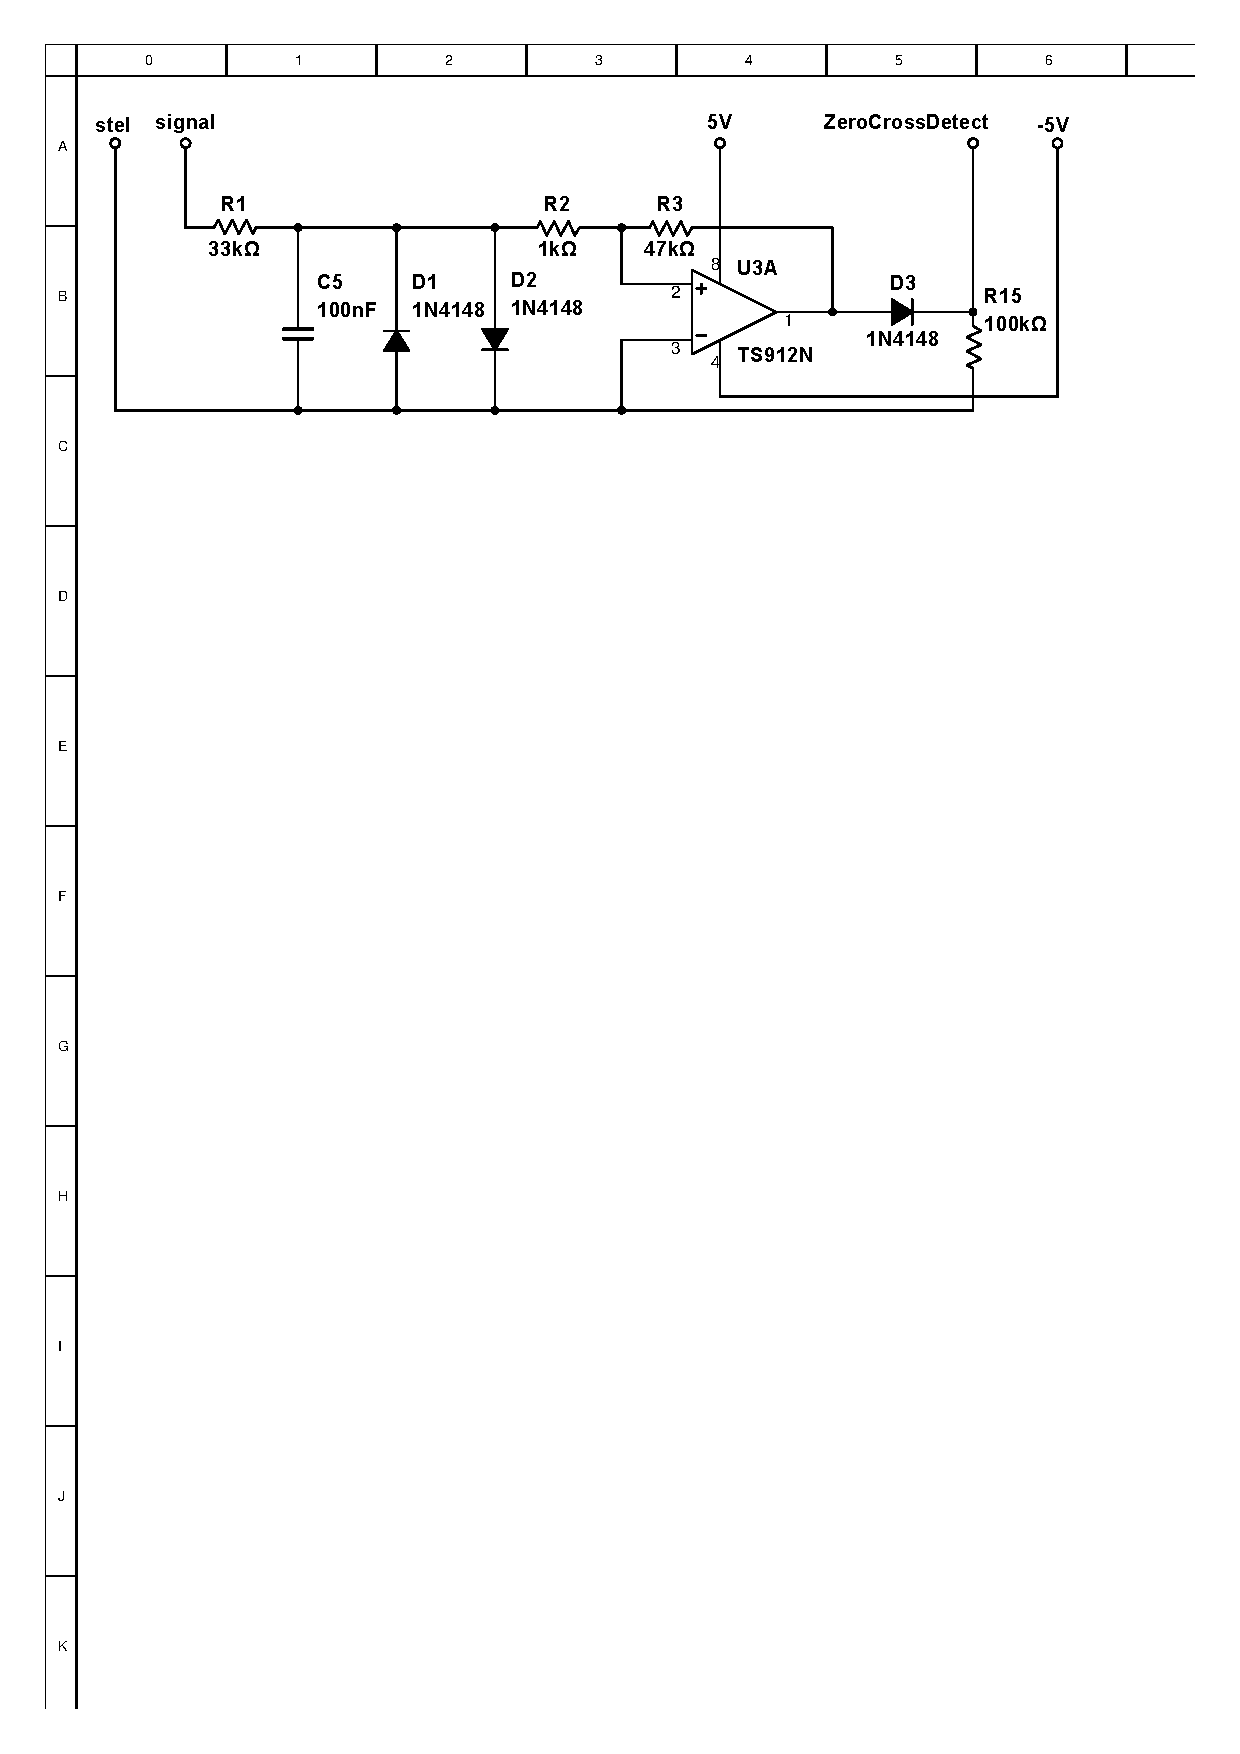
\includegraphics[scale=1, trim=45 635 80 50, clip=true]{../Projektdokumentation/HardwareDesign/Diagrammer/ZeroCrossDetector.pdf}
	\caption{Zerocross detector}
	\label{fig:ZeroCrossDetect}
\end{figure}

Kredsløbet består fra venstre mod højre af et lavpasfilter, to dioder\cite{lib:1N4148} til at begrænse spændingen, en operationsforstærker opsat som komparator med hysterese, en ensretter og en pull-down-modstand.\\

Det er valgt at bruge et lavpasfilter for at forhindre de $120kHz$, som også vil være til stede på \textit{signal}, i at genere kredsløbet ved at skabe ekstra nulgennemgange. Dioderne $D_{1}$ og $D_{2}$ begrænser spændingen til ca. $0.7V$, så vi ikke risikerer at ødelægge operationsforstærkeren ved at sende hhv. $\pm 25V$ ind på den.\\
Vi har valgt at bruge operationsforstærkeren TS912N, da denne kan forsynes med hhv. $\pm 5V$. Operationsforstærkeren\cite{lib:TS912} er opsat som komparator, således at den har $+5V$ på udgangen, hvis spændingen på plusbenet er højere end spændingen på minusbenet(referencespændingen), der er sat til $0V$. Hvis spændingen på plusbenet er lavere end referencespændingen, vil udgangen have en spænding på $-5V$. Der er tilføjet en hysterese med en passende størrelse ved hjælp af $R_{2}$ og $R_{3}$, for at undgå prel på operationsforstærkerens udgang.\\
Dioden $D_{3}$ ensretter strømmen, således at spændingen ikke kan blive negativ. Pull-down-modstanden $R_{15}$ trækker spændingen til $0V$, når udgangen på operationsforstærkeren er negativ, da det under implementering viste sig at være nødvendigt. Uden pull-down-modstand var signalet \textit{ZeroCrossDetect} ikke stabilt.\\

Efter de få nævnte tilpasninger, viste modul- og integrationstest, at kredsløbet virkede efter hensigten.

\newpage

\subsubsection{Carrier Generator}
Dette kredsløb har til formål at sende $120kHz$ signalet ud på $50Hz$ nettet. Dette skal ske uden at trække en væsentlig mængde strøm fra det STK500-kit, der generer de $120kHz$. Kredsløbets design vises på Figur \ref{fig:CarrierGen}. \\

\begin{figure}[h]
	\centering
	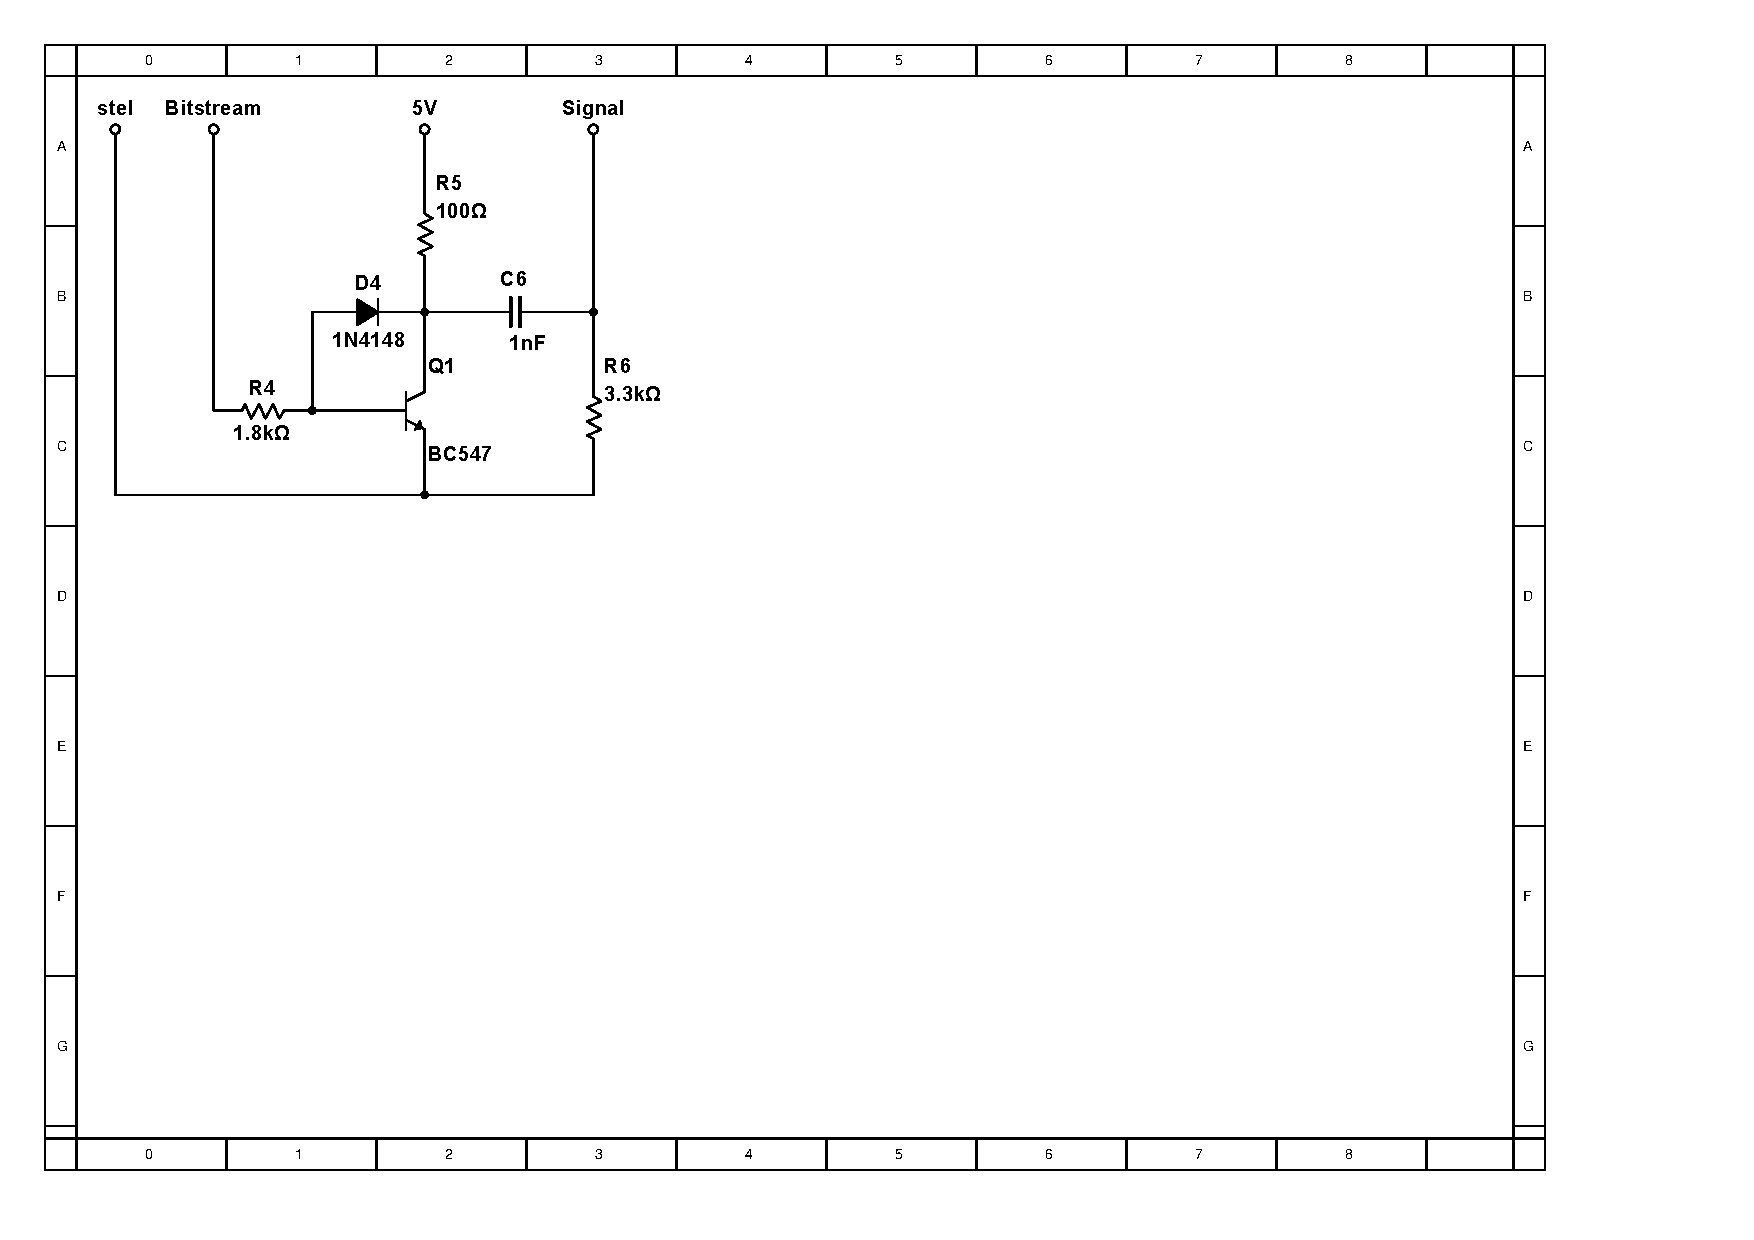
\includegraphics[scale=0.9, trim=45 355 525 45, clip=true]{../Projektdokumentation/HardwareDesign/Diagrammer/CarrierGenerator.pdf}
	\caption{Carrier generator}
	\label{fig:CarrierGen}
\end{figure}

Kredsløbet består af et transistor-kredsløb\cite{lib:BC547} og et højpasfilter($C_{6}$ og $R_{6}$). Højpasfilteret sikrer at transistor-kredsløbet ikke generes af $50Hz$ nettet, men $120kHz$ signalet, kan passere frit igennem. Transistor-delen, sørger for at åbne og lukke, for adgang til stel, i samme frekvens som \textit{Bitstream}, da transistoren er i mætning, hvilket bevirker at der er samme frekvens på collectorbenet som på basebenet af transistoren, men at strømmen trækkes fra $5V$ benet.\\

Transistoren BC547 er valgt, da denne har et lille storage delay. Målinger under implementeringen viste, at en positiv ladning af den transistor, der oprindeligt blev anvendt(BC139) ikke kunne nå at aflade, inden næste periode af $120kHz$ signalet skulle passere. Dioden $D_{4}$ hjælper ligeledes med at aflade den positive opladning af transistoren. Der er tale om en såkaldt baker clamp \cite{lib:BakerClamp}.\\

En modultest viser, at når \textit{Bitstream} har passeret gennem hele kredsløbet, er der påtrykt et $120kHz$ signal på $50Hz$ nettet. Signalet er ikke et ''pænt'' firkantsignal længere, og det har ikke en amplitude på $5V$, grundet diverse spændingsfald. Dette har ikke nogen betydning grundet carrier detectorens design. Der henvises i øvrigt til side \pageref{P-fig:CGImpl1} i projektdokumentationen for hele modultesten.\\

\newpage

\subsubsection{Lysmodul}
Lysmodulet har til formål at styre lysstyrken af en LED ved hjælp af pulsbreddemodulation (PWM). Dette gøres ved hjælp af en transistor\cite{lib:BD139} i mætning, således at middelstrømmen kan styres igennem LED'en, uden at strømmen trækkes fra STK500-kittet, som leverer \textit{lightPWM}-signalet. Kredsløbet er vist på Figur \ref{fig:Lysmodul-kredslob}.\\

\begin{figure}[h]
	\centering
	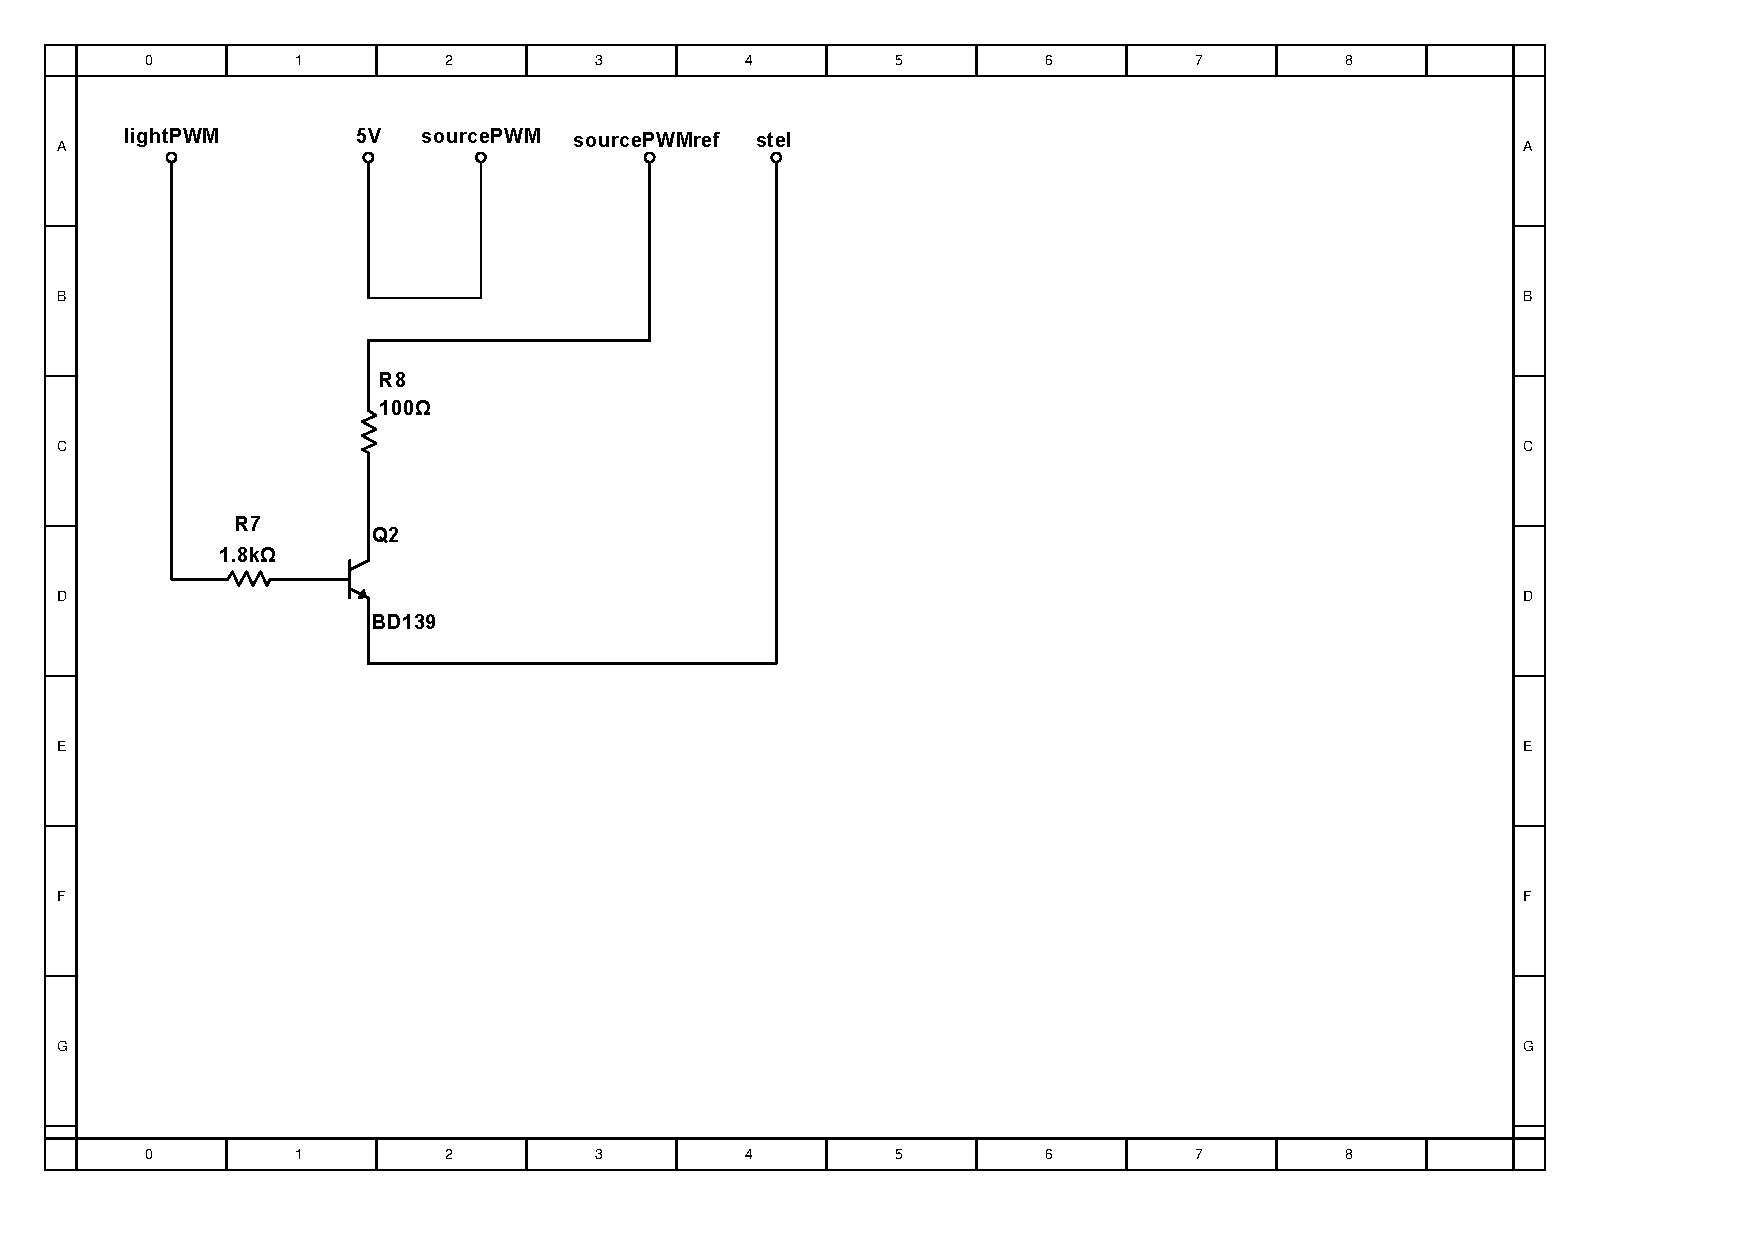
\includegraphics[scale=0.8, trim=50 250 440 60, clip=true]{../Projektdokumentation/HardwareDesign/Diagrammer/Lysmodul.pdf}
	\caption{Lysmodul}
	\label{fig:Lysmodul-kredslob}
\end{figure}

På terminalerne \textit{sourcePWM} og \textit{sourcePWMref}, tilsluttes den eksterne LED\cite{lib:LED}, som beskrevet i systemarkitekturen i projektdokumentationen på side \pageref{P-subsec:IBDX10Lys}.\\

Modul- og integrationstest af komponenten viser, at der tydeligt kan ændres i lysstyrken ved at ændre på duty cycle'en.\\

\newpage

\subsubsection{Carrier Detector}
Carrier detector'en har til formål at detektere, om et $120kHz$ signal er til stede på $50Hz$ nettet. Når et $120kHz$ signal er til stede på \textit{signal}, er udgangen \textit{Bitstream} HIGH, og hvis der ikke er et $120kHz$ signal til stede, er udgangen LOW. Kredsløbet er vist på Figur \ref{fig:CarDetek}.

\begin{figure}[h]
	\centering
	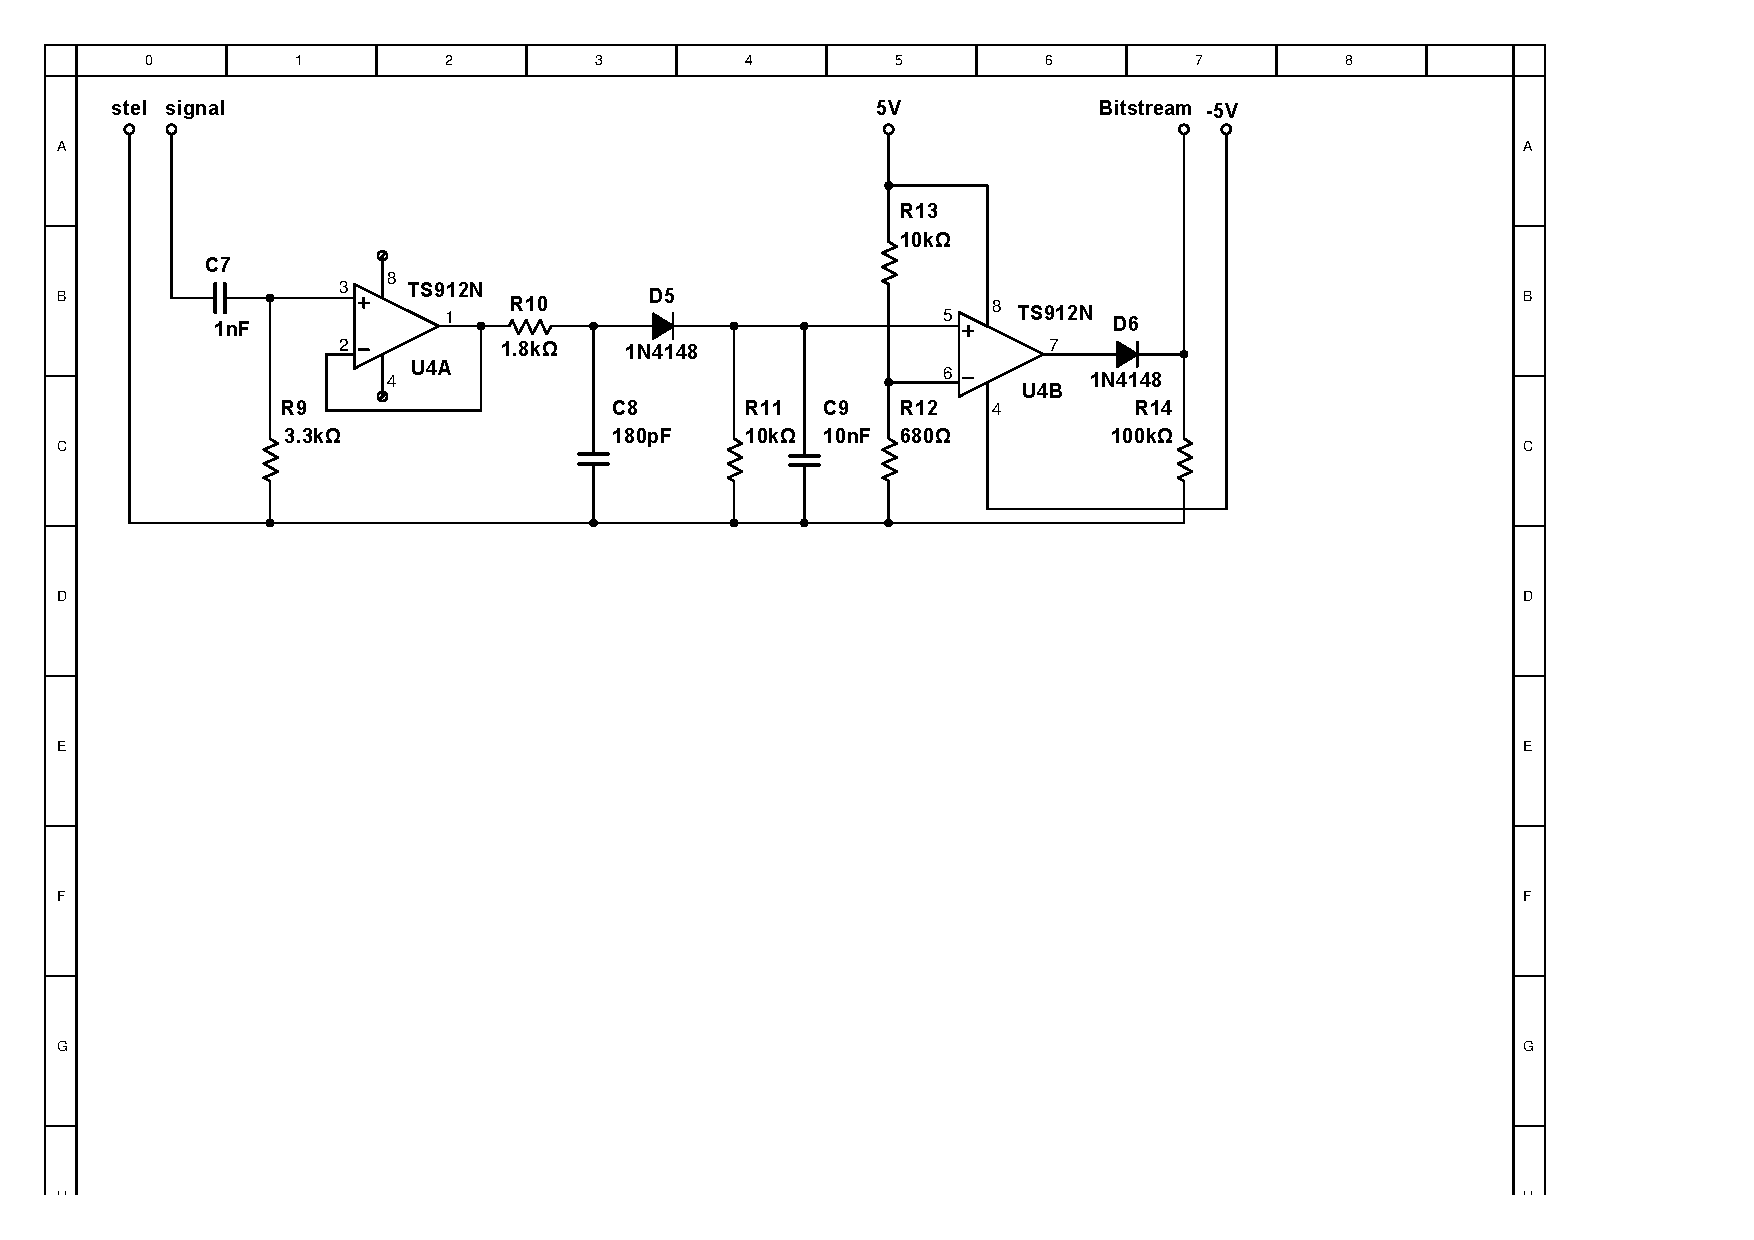
\includegraphics[width=\textwidth, trim=40 340 240 40, clip=true]{../Projektdokumentation/HardwareDesign/Diagrammer/CarrierDetector.pdf}
	\caption{Carrier detector}
	\label{fig:CarDetek}
\end{figure}

Fra venstre mod højre består kredsløbet af et båndpasfilter, en envelope detector, en operationsforstærker\cite{lib:TS912} opsat som komparator, en diode som ensretter og en pull-down-modstand.

Båndpasfilteret er designet, så det dæmper alle frekvenser på nær dem der ligger mellem $50kHz$ og $500kHz$, således at det frasorterer $50Hz$ og lader $120kHz$ passere. Da der er tale om et båndpasfilter, vil det også frasortere evt. højfrekvent støj, og evt. andre frekvenser end grundfrekvensen i $120kHz$ signalet. Det vil således være en tilnærmelsesvis sinus/cosinus, på $120kHz$, der lukkes igennem filteret.

Envelope detector'en består af $D_{5}$\cite{lib:1N4148}, $R_{11}$ og $C_{9}$ og har til opgave at holde spændingen omkring den positive peak-værdi, der er på $120kHz$ signalet. Dioden ensretter strømmen, således at det kun er positive spændinger der kan passere. Hvert peak af inputtet vil oplade kondensatoren, der sørger for, at spændingen i punktet mellem dioden og kondensatoren holdes nær peakværdien. Modstanden i parallel med kondensatoren vil gradvist aflade kondensatoren. Størrelserne på kondensatoren og modstanden er afpasset således, at afladningen sker i et passende tempo.

Operationsforstærkeren\cite{lib:TS912} er designet som en komparator, der har en udgangsspænding på $+5V$, når spændingen på ikke inverterende indgang er højere end spændingen på den inverterende indgang(referencespændingen). Når spændingen på ikke inverterende indgang derimod er mindre referencespændingen, er udgangsspændingen $-5V$. Referencespændingen er fastsat til en passende værdi, så spændingen på den ikke inverterende indgang kun er over spændingen på den inverterende indgang, når envelope detectoren detekterer et $120kHz$ signal.

Efter komparatoren er der placeret en diode $D_{6}$\cite{lib:1N4148}, som fungerer som ensretter, og en pull-down-modstand $R_{14}$, så der fremkommer et signal, der er i overensstemmelse med systemarkitekturen.

Modul- og instrumentationstest har vist, at komponenten virker efter hensigten. Spændingen på udgangen \textit{Bitstream} er ca. $4.7V$, når der er $120kHz$ til stede på \textit{signal}, og $0.0V$ når der ikke er $120kHz$ til stede på \textit{signal}.
\section{Software Design og Implementering}

I projektet er det valgt at programmere i C++ frem for C. På microcontrolleren fås den store fordel at koden kan opbygges i klasser frem for frie funktioner. ATMega32 microcontrolleren er valgt, pga. kendskab til netop denne via MSYS på første semester. Encapsulation fra C++ giver bedre sikkerhed for fejl, da det har været muligt, at tilgå member-data via mutator/accessor metoder. 

Det første tiltag under designfasen var angående, hvad design dokumentet skulle indeholde. Der blev udarbejde nogle klassebeskrivelser udfra applikationsmodelen på side \pageref{P-fig:PC_klasse} i dokumentationen. Da klassebeskrivelserne var lavet, blev der skrevet metodebeskrivelser til dem, så det var klart hvilke funktionaliter, returværdier og parameter lister metoderne skulle indeholde.
Under forløbet blev arbejdet opdelt, og uddelegeret under en modificeret version af Scrum.

Derefter blev proktokollen mellem boundary klasser udformet, så ingen misforståelser ville ske for de personer, som skulle implementere hver sin del af domæneområdet. Protokollen blev holdt så simpel som muligt, da fejl over kommunikationsmediet skulle minimeres.

\subsection{PC Domæne}

\begin{figure}[h]
	\centering 
	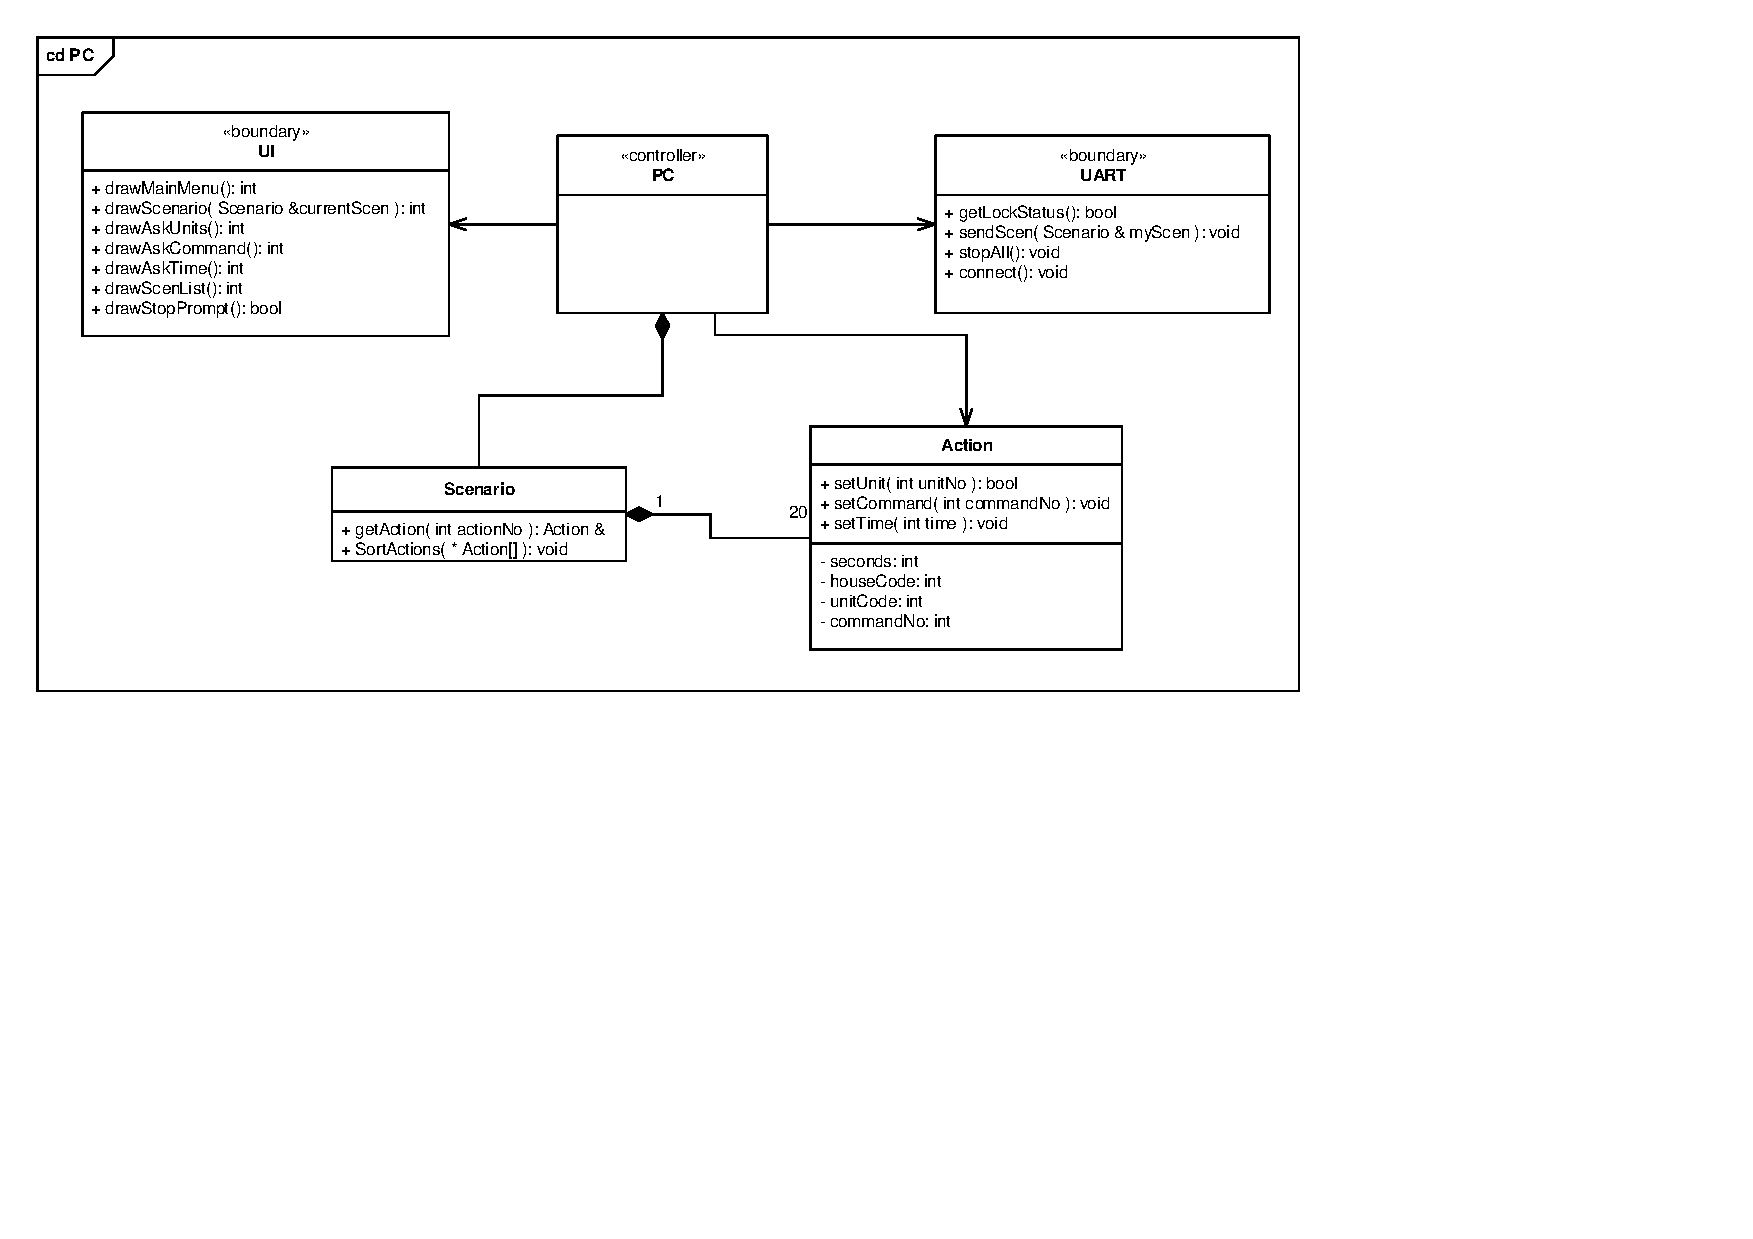
\includegraphics[width=\textwidth,trim=17 260 200 15, clip=true]{Projektbeskrivelse/Design_SW/diagrammer/PC_KlasseDiagram.pdf}
	\caption{Klassediagram for PC domænet}
\end{figure}

\texttt{PC Main} er ikke en klasse, men derimod den proces der sker når programmet eksekveres. Den har til opgave at kalde de rigtige metoder fra UI-klassen og gemme de data, den får fra brugeren ind i det korrekte actions objekt.
PC Main har også til opgave at transmittere data fra Scenariet, fra Scenario objektet, over til transmitteren ved brug af UART klassen.

\texttt{UART}-klassen har funktionaliteten til at sende strenge af data over til transmitteren igennem et RS232 kabel. Den har også mulighed for at kunne modtage respons fra transmitteren, når den skal have status på kodelåsen, som er tilknyttet transmitteren. UART'en oversætter den hentede data fra actions objekterne, så de følger protokollen for UART transmitteringen.
UART'en gør brug af et open source RS-232 biblioteket \cite{lib:UART}, og bruger dens funktioner til at forbinde til en gyldig COM-port, og sende og modtage data.

\texttt{Scenario}-klassen bruges til at holde de 20 actions objekter i. Den kan bruges til at hente de enkelte aktioner ud til manipulation og udskrivning af aktionerne på skærmen.
Scenario-klassen har også en sorteringsfunktion til at sortere aktionerne efter tid, så den tidligste tid står øverst og seneste tid nederst.

\texttt{Action}-klassen er til lagering af data, vedrørende hvad der skal ske på systemet. Ved brug af get- og set-metoder kan der manipuleres med dataen, så de kan tilpasses til den ønskede handling.

\texttt{UI}-klassen bruges til at have brugerinterfacet med på skærmen. Hver metode i klassen har til formål at fjerne tidligere indhold på skærmen, og tegne den nye menu. Efter menuen er på skærmen, har hver metode til formål at validere det input der kommer fra brugeren, og returnere informationer når gyldigt input registreres. UI klassen er den eneste mulighed brugeren har for at styre systemet på.

  
\subsection{Transmitter Domæne}

\begin{figure}[h]
	\centering \resizebox{\textwidth}{!}{
	\includegraphics[scale=0.5,trim=17 200 180 15, clip=true]{Projektbeskrivelse/Design_SW/diagrammer/Transmitter_KlasseDiagram.pdf}}
	\caption{Klassediagram for transmitter domænet}
\end{figure}

\texttt{Transmitter}-klassen holder styr på, at de forskellige klasser kan snakke sammen. Den indeholder også alle de actions, som bliver overført via UART'en.

\texttt{Codelock}-klassen tjekker, om koden er indtastet rigtigt på DE2 bordet.

\texttt{UART}-klassen kommunikerer med PC'en via UART, hvor der sendes informationer om status på codelock og der modtages scenarier fra PC'en. Her modtages 100 chars som svarer til 20 aktioner. Kommunikationsvejen er over RS232.

\texttt{Tx10}-klassen styrer alt kommunikation mellem transmitteren og receiverne, som foregår på el-nettet gennem X.10 protokolen. Timeren sørger for at sendes nøjagtigt i et milisekund.

\texttt{Action}-klassen holder styr på aktioner som skal køres på receiverne. Disse indeholder time, unit, command og house code så den ved hvor, de forskellige data skal sendes hen.

\texttt{Time}-klassen holder styr på tiden, så scenariet kan blive eksekveret til den ønskede tid. Timer1 bruges til at generere et interrupt hvert sekund, men det sendes kun videre til controlleren hver femte sekund for at være sikker på, at den kan nå at sende informationer over X.10 uden problemer. 

\subsection{Receiver Domæne}

\begin{figure}[h]
	\centering \resizebox{\textwidth}{!}{
	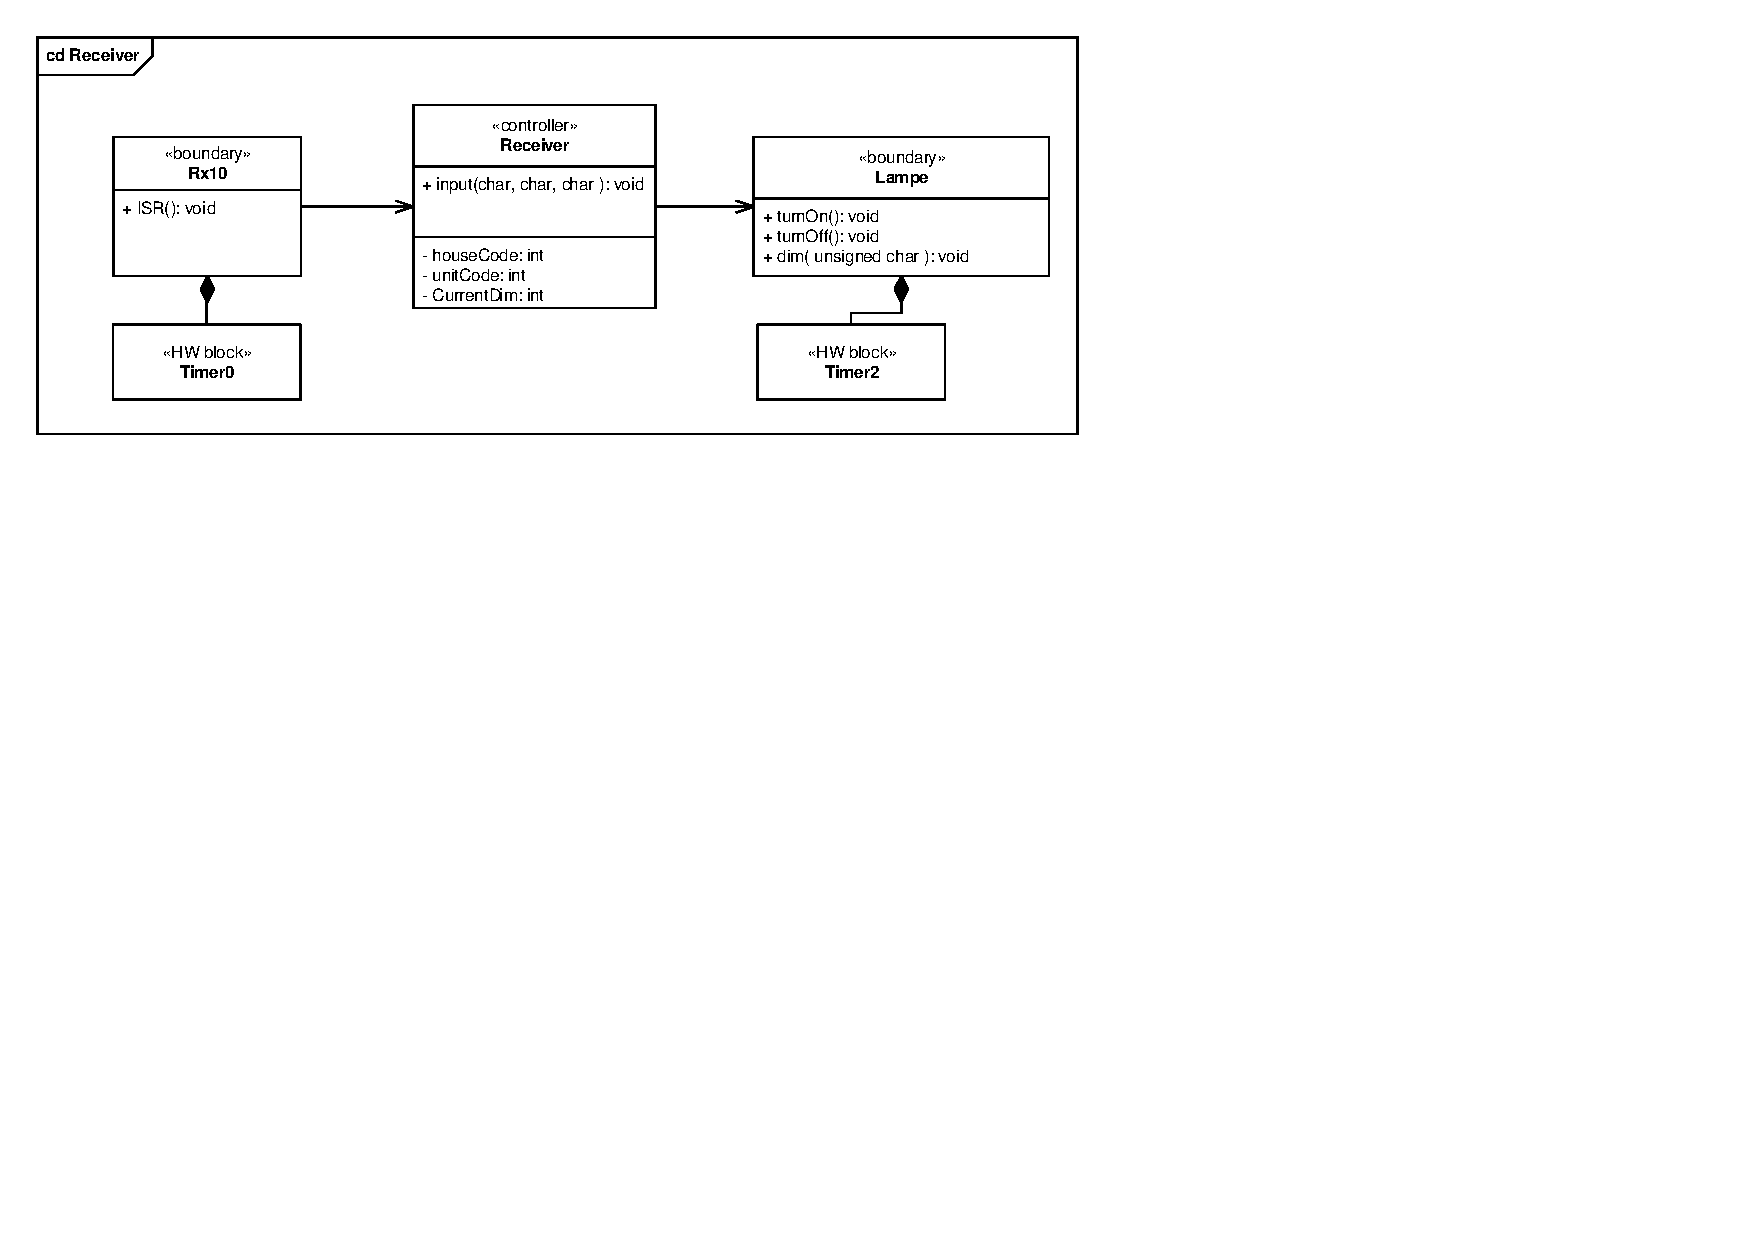
\includegraphics[scale=1,trim=17 380 320 18, clip=true]{Projektbeskrivelse/Design_SW/diagrammer/Receiver_KlasseDiagram.pdf}}
	\caption{Klassediagram for receiver domænet}
\end{figure}

\texttt{Rx10}-klassen er en boundary til Transmitter domænet, og har til opgave at modtage kommandoer fra X.10 nettet, samt formidle dem til receiver controller klassen.

\texttt{Timer0} er indbygget i ATmega32, og bruges af Rx10 klassen til at kontrollere for et 120kHz signal et halvt milisekund efter en nulgennemgang på 50Hz signalet.

\texttt{Receiver}-klassen manipulerer et Lampe objekt alt efter hvilken kommando der modtages.

\texttt{Lampe}-klassen styrer tænd, sluk og dim funktionaliteten.

\texttt{Timer2} bruges til at lave et variabelt PWM signal, der kan ændres af Lampe-klassen.


\subsection{Software Implementering}

Ved start af implementeringsfasen blev alle klasser skrevet ind på et Scrum-board, hvorefter hver udvikler kunne tage en opgave og gå i gang med at implementere den. Implementeringsfasen kørte som en iterativ procces, hvor softwareudvikleren først implementerede designbeskrivelsen og skrev modultest dertil. Dernæst blev klassen sendt til en delvis integrationstest, som er afhængig af dens funktionalitet. Se s. \pageref{P-TxUART} i dokumentationen.

Undervejs blev der fundet mangler og udnødvendige klasser i designbeskrivelsen. Ydermere skulle UART protokollen fra design revideres pga. fejl i modultesten. Fejlen var at værdien 'null' ikke kunne sendes med RS-232 biblioteket. Løsningen var at skifte fra '0-255' til '48-63', således at der kun er 16 brugbare værdier i hver sendt char istedet for 256. Skiftet resulteret i der nu skulle sendes 3 chars, istedet for 2 chars, til at overføre tiden for en enkelt aktion.

Der opstod problemer med at Rx10, fordi ''sladrehanks klassen'', se side \pageref{P-Rx} i dokumentation, var meget lang tid om at sende data ud af RS-232 porten. Problemet var at den ikke var interrupt baseret, og derfor hentede/sendte data hele tiden. 
\section{Integrationstest}
Under integrationen af de samlede moduler opstod der flere problemer, som blev løst gennem forskellige fejlsøgninger af det samlede system. Herunder vil de brugte testmetoder under integrationen blive forklaret.\\

For at kunne se hvordan enhederne i systemet kommunikerer, er der på de forskellige softwareenheder lavet funktioner, der kan ''sladre'' gennem UART-kommunikation. Dette sammen med programmet Tera Term(terminal) giver mulighed for at se præcis hvor i koden de individuelle enheder er. Et kode eksempel på dette kan ses på Figur \ref{fig:sladrehank}.\\

\begin{figure}[h]
	\begin{lstlisting}
...
	if (debugging)
	{
		getMyTxUART()->sendString("Checking time, current time is: ");
		getMyTxUART()->sendNumber(minutes);
		getMyTxUART()->sendChar(':');
		getMyTxUART()->sendNumber(seconds);
		getMyTxUART()->sendString("\n\r");
	}
...
	\end{lstlisting}
	\caption{Eksempel på en sladrehank fra Transmitter Time klassen}
	\label{fig:sladrehank}
\end{figure}

Det kan ske at koden fortæller, at den gør en ting, men i realiteten sker dette ikke. For at kunne analysere sådan et problem, er det ofte lettere at analysere direkte på rådata via kommunikationen. Her er oscilloskop'et et stærkt fejlsøgningsredskab, da det er muligt at se, hvad der sker direkte på kommunikationsvejen mellem de individuelle moduler. Ved analysering af spændingen på indgange og udgange af systemets individuelle enheder kan en fejl hurtigt indrammes om det er et hardware eller software problem. Et eksempel på rådata, der kan analyseres, kan ses på Figur \ref{fig:oscilloskop}.\\

\begin{figure}[h]
	\centering
	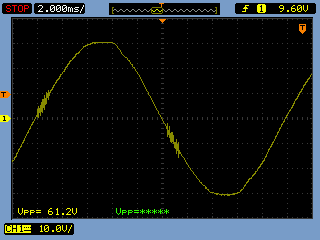
\includegraphics[scale=0.75, trim=0 0 0 0, clip=true]{Projektbeskrivelse/Integrationstest/billeder/Oscilloskop.png}
	\caption{Oscilloskop screenshot af X.10 på $18V AC$}
	\label{fig:oscilloskop}
\end{figure}

Med standard frekvens på $50Hz$ kan det være svært at analysere på systemet, da der sker to nulgennemgange for hver periode der kører. Dermed kan systemet kommunikere med $100$ bits i sekundet. For at komme uden om dette problem er der blevet testet med en lavere frekvens, helt ned til $1Hz$, under systemets integration. Dette gør det muligt at aflæse data på LED'er på STK500 kittene.
\section{Resultater og diskussion}
Projektet er endt ud med en prototype af et produkt, der med få undtagelser, bestod accepttesten. Det blev valgt ikke at implementere TV- og radiodelen af produktet, da det blev bestemt at fokus skulle ligge på det resterende system. De problemer og udfordringer der opstod under gennemførelsen af projektet, er blevet løst via et samarbejde i gruppen, hvor alle bidrog med viden og faglige kundskaber. De punkter som der i kravsspecifikationen blev sat fokus på, er blevet implementeret og systemet er stabilt, fejlfrit og fungerer selvstændigt.

Igennem projektperioden er der for hardware blevet lagt vægt på løsninger, der uden at være alt for komplicerede, kan klare deres opgaver som beskrevet. For at sikre stabile logiske niveauer i systemet, og dermed undgå prel, blev det valgt at implementere operationsforstærkere som komparatore med både positiv og negativ spændingsforsyning. Under implementeringen af hardware stødte gruppen på en del problemer, med de designs der var lavet på forhånd. Men med den rette vejledning, forblev projektet på sporet og endte ud med at have en tilfredsstillende prototype. I forhold til hvad der blev forventet af designet, har implementeringsprocessen været meget lærerig, da de problemer der opstod var med til at vise nye perspektiver på kredsløbene. Alle komponenterne blev realiseret på veroboard og testet hver for sig i modultests.

For softwaredelen var det vigtigt at få designet og implementeret noget enkelt men funktionelt kode. Processen har ledt til forståelse af, hvor vigtigt det er at have en test klar før selve kodningen af softwaren foretages. Softwaregruppen fandt desuden ud af, at det skal gøres helt klart hvilken klasse der skal gøre hvad og hvornår, for at undgå misforståelser mellem klasserne. Ved softwareintegration blev de dele af koden der var mulige at teste, som fx transtmitter UART'en, grundigt testet. Dog var det i andre tilfælde nødvendigt at vente til den samlede integrationstest, for at opdage de fejl der var på hhv. transmitteren og receiveren. 
Der blev konstrueret en såkaldt ”sladrehanks klasse”, der kunne fortælle hvad der sker under kommunikation med UART og over elnettet.

Integrationstesten var et afgørende punkt for projektet, da det er første gang det hele skulle sættes sammen. Der blev hurtigt fundet nogle fejl, som blev løst efterhånden. Stille og roligt begyndte systemet at fungere, som det blev designet til. Samarbejdet mellem software og hardware fungerede som det skulle, takket være en god planlægning af grænsefladerne mellem elementerne i systemet. For at finde de fejl der opstod, blev der sat en langsommere frekvens ind, i stedet for $50Hz$, og relevante outputs blev vist på LED’er, således det var muligt at aflæse hvad der blev sendt og modtaget. 

Det hele endte ud med en accepttest, som systemet bestod næsten uden undtagelser. Da det relativt tidligt i forløbet blev valgt ikke at implementere radio- og TV-delen, var det ikke muligt at bestå de tests der var opstillet for disse punkter. Systemet endte ud med at blive fejlfrit og meget sikkert, da det også blev testet med en væsentligt højere frekvens end $50Hz$ og stadig fungerede. Helt fra starten blev det vedtaget, at formålet med projektet var et simpelt system, og fokus skulle lægges på indlæring. Denne beslutning har gruppen værdsat højt, og har gjort at hvert medlem i gruppen har fået mest muligt ud af projektet.

\section{Opnåede Erfaringer}
\subsection{Fælles Erfaringer}
Der er bred enighed om at denne gruppe består af engagerede medlemmer. Engagemanget har til tider dog gjort, at ligegyldige detaljer har taget ekstra tid at diskutere, men derudover har gruppen været produktiv og god til at kommunikere. Der er en fælles holding om at de har gået en lærerig proces igennem og fået rigtige mange faglige erfaringer med sig gennem projektet.
\subsection{Henrik}
Dette semesterprojekt har været belærende på mange områder. Fagligt føler jeg, at jeg har fået rigtig meget ud af dette forløb. Jeg har hovedsageligt været en del af hardware gruppen og har derfor haft stort ansvar inden for hardware modulerne i projektet. Dette gør selvfølgelig at jeg har fået mest faglig viden inden for hardware. Jeg har sørget for også at få lidt arbejde i softwaremodulerne, dermed har jeg også fået en forøget faglig viden inden for software.\\
Jeg har for første gang i lang tid følt at jeg har været i en stærk gruppe. Der er dog både positive og negative sider ved dette, da der hurtigt kan opstå konflikt om irrelevante ting, fordi alle i gruppen altid udtaler deres mening. Men da dette er det værste, der er sket i gruppen, efter min mening, kan man ikke rigtig sige at der har været nogle direkte problemer i gruppen. Det største problem ved dette, for mig personligt, er at siden der er så mange der vil udtale deres meninger, har jeg i mange tilfælde prøvet at holde mig tilbage, da det blot ville mindske arbejdshastigheden, hvis jeg også altid udtalte mine meninger. Jeg har dog lært gennem dette, at selv hvis jeg har det på den måde, bliver jeg nød til at sige min mening, i det mindste for de vigtigste emner.
\subsection{David}

I dette projekt, havde jeg valgt at lave både hardware og software fordi det er sidste gang, hvor alle er lige med undervisning i alt. Næste semester bliver vi delt op også skal man nok i højere grad arbejde med den disciplin man vælger. Jeg synes godt det kunne være lidt svært at omstille sig når man hoppede fra disciplin til disciplin, men jeg er glad for at jeg gjorde det fordi jeg er blevet bedre til både hardware og software. Projektet har vært rigtig sjovt, man har kunnet se software og hardware gå op i en højere enhed og fungere sammen til sidst. Som gruppe har vi helt klart arbejdet rigtig godt sammen og haft det sjovt på samme tid.
\subsection{Morten}
Arbejdet med dette projekt har for mig været meget lærerigt. 
Jeg har fået et højt fagligt udbytte, særligt i design og implementeringsfaserne. 
Den størte læring ligger dog, efter min mening, i selve processen. Det har været en udfordring at indgå i en projektgruppe med ene engagerede medlemmer. 
Ofte har vi brugt lang tid på at diskutere mere eller mindre ligegyldige ting, fordi de enkelte medlemmer - inklusive jeg selv - holdt hårdt på egne holdninger og meninger. 
Dette er sket mindre og mindre i løbet af projektarbejdet.

Jeg føler at jeg særligt har lært meget inden for styring og koordinering af et større projekt. 
Det er naturligvis helt essentielt, at der er styr på hvem der gør hvad, i hvilken rækkefølge og hvornår det skal være klar. 
Jeg synes at vi som gruppe har klaret den udfordring ganske udmærket, og jeg mener, jeg har bidraget positivt hertil. 

\subsection{Kristian S.}

Gennem arbejdet har jeg opnået en bedre forståelse af, hvordan større projekter skal struktureres, her tænker jeg særligt på SysML og Scrum. Fagligt har mit fokus været på software udvikling især med brug af C++ Standard Template Library(STL), hvor brugen af vector containeren og sort funktionen i algorithm har forenkelt en del arbejde. Generelt er mit indtryk at samarbejdet i gruppen har fungeret meget fint, f.eks. var tidplanen kun blevet revideret en gang. Med min nuværende viden vil noget lidt mere forarbejde give bedre tid i enden.
\subsection{Kasper}
Semesterprojektet har været en rigtig god måde at bruge de lærte fagligheder fra andre fag i. Det har givet mulighed for at bruge det lærte stof fra fagene på semesteret til at realisere vores eget produkt. At arbejde med PC-UARTen har givet mig en større forståelse og færdighed indenfor brug af opensource biblioteker til programmering af områder jeg ikke selv har færdighederne til at skrive fra bunden.
Samarbejdet har været godt, men der har indimellem været nogle lange diskussioner omkring små, ret ubetydelige ting. Det har dog samtidig ført til en solid dokumentation, og gjorde design og integration nemt at arbejde med. 
\subsection{Philip}
Projektarbejdet har været meget lærerigt, både inden for de fag, der indgår i projektet, men også hvad angår selve processen i arbejdet. Jeg har fået øjnene op for det store udvalg af værktøjer der findes til strukturering og planlægning af projektarbejdet. De værktøjer har vi i gruppen anvendt flittigt igennem forløbet. Jeg har derfor fået nogle gode erfaringer, som jeg kan bruge i de kommende projekter. Her tænker jeg bl.a. på anvendelse af Scrum-elementer, tidsplan mm.
I gruppen har alle arbejdet flittigt og været engagerede. Det har til tider været trættende og har langsommeliggjort arbejdet, da alle, inklusiv jeg selv, har haft en holdning og gerne vil bidrage til det stof, vi i fællesskab, har arbejdet på. Her kræver det selvdisciplin fra min side, hvis jeg i fremtiden skal blive bedre til at undlade at bringe små og ligegyldige ændringsforslag på bordet.

I dette projektforløb har jeg næsten udelukkende beskæftiget mig med hardware, hvor der har være meget at tage fat på. Jeg har arbejdet med design af filtre, design af komparatorer, generel signalbehandlelig og ikke mindst fejlsøgningen. Jeg synes resultatet er blevet godt, hvilket jeg tror skyldes det simple design vi har holdt.
\subsection{Lasse}
Gennem hele projektet har vi lagt vægt på at lære mest muligt, hvilket virkeligt har udvidet min horisont mht. de problemer det har lykkedes os at løse. Desuden har vores fordeling af arbejde på både software og hardware været rigtig god - altså at alle har kunnet arbejde på hvad de vil. Vi tog et valg tidligt i forløbet omkring at bruge LaTeX som skriveprogram, hvilket jeg er meget positivt overrasket over. Alt i alt synes jeg projektet og dermed også gruppearbejdet har forløbet fint. Det har været en spændende proces at skulle væne sig til at arbejde i en ret seriøs gruppe, hvor der har været meget på tallerkenen fra start, men det har været besværet værd. Udbyttet af dette projekt er for mig personligt meget større end det var i forrige projekt. Set i bagspejlet har det været en fornøjelse at arbejde med 2. semesterprojekt. 
\subsection{Kristian T.}

På trods af at vi har valgt at lave et relativt simpelt projekt i forhold til den stillede opgave, har dette projekt været meget lærerigt for mit vedkommende. 
Jeg har specielt haft meget gavn af selve processdelen, hvor vi i vores gruppe har haft meget stor engagement i forhold til projektet, det har jeg ikke været vant til fra tidligere projektgrupper.
Jeg har lært at der er store fordele ved at planlægge selve omfanget af projektet rent praktisk i forhold til at have styr på udformning af afsnit i de forskellige dokumenter samt styring af fildeling. 

Under dette projekt har jeg været ansvarlig for at holde styr på vores Dropbox, hvor vi bl.a. har haft alle .tex filer til projektdokumentation og rapport samt alle filer til figurer, der skulle inkluderes i disse.
Dette har medført at jeg har gjort mig en del erfaringer omkring organisation af et større dokument med mange filer, der skal hæftes sammen, og placering af figurer i forhold til disse.
Bl.a. er det en god idé at være foran med planlægningen af kommende dokumenter, så det er klart hvor de øvrige medlemmer i gruppen skal finde det relevante materiale.

Jeg føler generelt at vi har haft en rigtig godt samarbejde i gruppen med en klar vision om hvad vi ville nå frem til og jeg har lært en masse at tage med på de efterfølgende semestre. 

\section{Fremtidigt Arbejde}
Under dette projekt er der mulighed for at færdiggøre og udvikle det ønskede produkt. Der har gennem projektets fremgang været tænkt på forskellige idéer, der ville kunne gøre dette system bedre.

Der blev, som dokumenteret under projektafgrænsning, bestemt at dette projekt ikke ville færdigudvikle TV- og Radio-forbindelserne til systemet. Dette ville selvfølgelig være en mulighed for at forbedre systemet.

Ud over det basale i at færdiggøre projektets første idéer, ville en optimering og fysisk indkapsling af produktets enheder være idéelt. Dette ville herefter kunne videreudvikles til at lave produktet ren modulbaseret, således at det er muligt at koble flere eller færre enheder til systemet så det kan tilpasses den individuelle persons behov.

Systemets kommunikation er envejs-baseret. Udvidede man dette til en tovejskommunikation, ville det kunne mindske risiko for fejl, samt give muligheden for at kunne kommunikere med systemet fra de forskellige enheder i systemet, frem for at være begrænset til den primære microcontroller.

Softwaren er efter integrationsfasen fyldestgørende, men har rig mulighed for at blive opdateret med flere funktionaliteter og en eventuelt grafisk user interface. Udover dette ville softwaren ligesåledes kunne udvikles således at det kan kommunikeres til og fra andre enheder såsom en smartphone, via f.eks. en smartphone app.
\clearpage
%   
\documentclass[a4paper,11pt,oneside,article]{memoir}
\renewcommand{\baselinestretch}{1.05}
\usepackage{amsmath,amsthm,verbatim,amssymb,amsfonts,amscd, graphicx}
\usepackage{graphics}
\usepackage[utf8]{inputenc}
\usepackage[danish]{babel}
\topmargin0.0cm
\headheight0.0cm
\headsep0.0cm
\oddsidemargin0.0cm
\textheight23.0cm
\textwidth16.5cm
\footskip1.0cm
\theoremstyle{plain}
\newtheorem{theorem}{Theorem}
\newtheorem{corollary}{Corollary}
\newtheorem{lemma}{Lemma}
\newtheorem{proposition}{Proposition}
\newtheorem*{surfacecor}{Corollary 1}
\newtheorem{conjecture}{Conjecture} 
\newtheorem{question}{Question} 
\theoremstyle{definition}
\newtheorem{definition}{Definition}

\begin{document}

\frontmatter

\title{Latex}

\author{Kristian}

\maketitle

\clearpage

\mainmatter

\chapter{Brug af LaTex}

\begin{enumerate}

 \item Åben Template.tex med texmaker.
 
 \item Tryk F1, og texmaker begynder en "quick build". Du burde nu se et vindue med din pdf, ellers tryk F1 igen.
 
 \item Over i din tex fil, vil du se \textbackslash title \{ Latex \} . Erstat "Latex" med "Mit første latex dokument" og tryk F1.
 
 \item Du kan kan gøre det samme med \textbackslash author \{ mit navn \} og tryk F1 igen. 
 
\end{enumerate}

(Du behøver ikke trykke F1 efter hver lille ændring) 


\chapter{Layout}

\section{Sections og subsections}

Latex består af kapitler og sektioner (og derunder undersektioner og underundersektioner). Formatet er det samme, $\backslash chapter \{ Something \}$, Hvor "Something" er navnet på din afsnit. Prøv at indsætte $\backslash chapter \{ Something \}$ under $ \backslash maketitle$ i din tex dokument og tryk F1. \\
\\
Du kan også lave afsnit med $\backslash section \{ Something else \}$. Prøv at indsætte 
$\backslash section \{ Something else \}$ under $\backslash chapter \{ Something \}$ i din tex dokument og tryk F1. \\
\\
Under $\backslash section \{ Something else \}$ kan du skrive din tekst til afsnitet. Prøv at skrive en lille tekst, og derefter compile med F1.\\
\\
Du kan ligeledes lave underafsnit med $\backslash subsection \{Something \}$ og underunder afsnit med $\backslash subsubsection \{Something \}$. Du behøver ikke lave afsnit eller underafsnit for at skrive brød tekst, men det ser bedre ud.

\section{Newpage og newline}

Hvis du gerne vil starte på en ny side, så skriv $\backslash newpage$.

Ønsker du at lave en ny side, hvor floats (billeder, tabeller etc.) ikke følger med fra de forrige sider, bruger du $\backslash clearpage$. \\

$\backslash \backslash$ efter en linie tekst giver en newline.

\newpage

\chapter{Billeder/tabeller}

\section{Import billeder}

\begin{enumerate}

	\item Find et billede, du gerne vil indsætte, og læg det i samme mappe som din tex fil.

	\item Under din lille tekst fra forrige øvelse indsæt $\backslash includegraphics[scale=1]{pic.png}$
	
	\item Erstat pic.png med navnet på dit billede (husk at tilføre fil- typen på dit billede som vist i 		  eksemplet) 
	
	\item Scale sætter hvor stort billedet skal være, Så scale=0.5 sætter billedet til halv størrelse.

\end{enumerate}


\section{Tabel}

Skriv en sandhedstabel for en AND-gate. \\
\\
Brug http://en.wikibooks.org/wiki/LaTeX til at finde ud af hvordan tabeller laves.

\chapter{Matematik}

Matematiske formler kan skrives på flere forskellige måder. \$ math formel \$ giver et "matematikfelt" in-line, dvs det kan skrives i brødteksten. $\backslash begin \{ displaymath \}$ giver et matematikfelt på sin egen linie og i midten. $\backslash begin \{ equation \}$ gør ca det samme som $displaymath$, men giver linien et nummer, som man kan sætte en label på med $\backslash label \{something \}$ og derefter referere til med $\backslash ref \{something \}$. Indskriv \\
 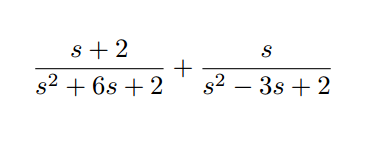
\includegraphics[scale=1]{../lektion/math.png} \\
i latex vha. http://en.wikibooks.org/wiki/LaTeX/Mathematics.


\end{document}
\chapter{Konklusion}
Overordnet set opfylder projektarbejdet fuldstændigt opgavens mål og formål inden for de rammer, der er givet i projektoplægget. 
Der er blevet designet og realiseret et system, som kan forebygge indbrud i en bolig. 
De dele af systemet, der er blevet realiseret, fungerer stort set fejlfrit og meget stabilt. 

Det besluttedes fra starten at systemet skulle være så simpelt som muligt, hvilket med sikkerhed har medvirket til det gode resultat. 
Heri ligger en af de vigtigste erfaringer i projektarbejdet. 
Denne beslutning gennemstyrer hele projekarbejdet og det gælder således, at såvel HW som SW er forsøgt designet og implementeret så simpelt som muligt.
Det er dog klart at man er nødt til at gå på kompromis med ekstra funktionalitet, fejlsikring mm., hvilket har stillet projektgruppen overfor nogle vigtige beslutninger undervejs i forløbet. 
Det er undervejs i forløbet fx ofte blevet nævnt, at ''...det ville have været rart med tovejskommunikation'' på elnettet. 
Havde vi implementeret dette, kunne vi have sikret os mod fejl ved simpelthen at sende en kommando igen, hvis den ikke blev modtaget. 
Vi har dog ikke oplevet decideret behov herfor; X.10 kommunikationen på elnettet fungerer fejlfrit.

En mindst ligeså vigtigt læring ligger inden for styring af processen. 
Vi har efter vores egen mening formået at styre projektforløbet særdeles godt. 
Der har undervejs kun været behov for at rette i tidsplanen enkelte gange, og dokumentation er blevet skrevet og opdateret løbende. 
Dette har betydet at der har været god tid i de sidste faser og god tid til at skrive rapport. 

Projektgruppen har udviklet sig meget under projektforløbet. 
Gruppen havde ikke arbejdet sammen som helhed før, og der var som forventeligt lidt udfordringer i starten.
Det var særdeles fornuftigt at starte med at lave en samarbejdsaftale, og derigennem få afstemt forventninger til arbejdet og systemet.  
Alle gruppemedlemmer var fra starten meget engagerede, hvilket betød at gruppen ofte måtte bruge en del ressourcer på at blive enige om forskellige beslutninger. 
Efterhånden som projektarbejdet er skredet frem, og gruppemedlemmerne har fundet deres roller i gruppen, er samarbejdet blevet mere og mere strømlinet. 
Der er stadig plads til yderligere udvikling, såfremt samarbejdet fortsættes.

\clearpage
\renewcommand{\bibname}{Litteraturliste}
%\chapter{Litteraturliste}
\begin{thebibliography}{2}

\bibitem {lib:LM7805} Fairchild: \textit{LM7805 datasheet}. "Bilag 017 - LM7805". 2006.

\bibitem {lib:IC7660} Maxim: \textit{IC7660 datasheet}. "Bilag 018 - IC7660". 1994.

\bibitem {lib:1N4148} NXP: \textit{1N4148 datasheet}. "Bilag 019 - 1N4148". 2010.

\bibitem {lib:TS912} Farnell: \textit{TS912 datasheet}. "Bilag 020 - TS912". 2012.

\bibitem {lib:BC547} Fairchild: \textit{BC547 datasheet}. "Bilag 021 - BC547". 2002.

\bibitem {lib:BD139} Fairchild: \textit{BD139 datasheet}. "Bilag 022 - BD139". 2007.

\bibitem {lib:LED} Kingbright: \textit{L-53-YD 5mm datasheet}. "Bilag 023 - L-53-YD 5mm". 2006.

\bibitem {lib:AtMega32} Atmel: \textit{ATMega32 datasheet}. "Bilag 024 - ATMega32". 2011. 

\bibitem {lib:Adaptor} Mascot: \textit{8610 AC/AC adaptor}. "Bilag 010 - 8610AC Adaptor". Ukendt årstal.

\bibitem {lib:UART} Beelen, Teunis van: \textit{RS-232 for Linux, FreeBSD and Windows}. \url{http://www.teuniz.net/RS-232/}. 2014-12-11.

\bibitem {lib:AN236} Burroughs, Jon: \textit{AN236}. "Bilag 011 - AN236". 2002.

\bibitem {lib:Codelock} Krogh-Pedersen, Philip: \textit{Kode fra Exercise 7.2 DSD}. "Bilag 012 - Codelock". 2014.
 
\bibitem {lib:Samarbejdsaftale} Gruppe 1: \textit{Samarbejdsaftale}. "Bilag 013 - Samarbejdsaftale". 2014.

\bibitem {lib:Moedereferater} Gruppe 1. \textit{Mødereferater PRJ2}. "Bilag 014 - Mødereferater". 2014.

\bibitem {lib:AtMega32sum} Hargaard, Henning: \textit{Summary from the Atmel Mega32 manual}. "Bilag 016 - AtMega32 summary". 2011.

\bibitem {lib:Testscenarie} Gruppe 1: \textit{Testscenarie-dokumentet}. "Bilag 003 - Testscenarie-dokumentet". 2014.

\bibitem {lib:ColorPix} ColorSchemer: \textit{ColorSchemer - Free screen color picker from ColorSchemer}. \url{http://www.colorschemer.com/colorpix_info.php}. 2014-12-14.

\bibitem {lib:BakerClamp} Wikipedia: \textit{Baker clamp}. \url{http://en.wikipedia.org/wiki/Baker_clamp}. 2014-12-11.

\bibitem {lib:atmel} Atmel: \texttt{C++ compiling}. \url{http://www.atmel.com/webdoc/AVRLibcReferenceManual/FAQ_1faq_cplusplus.html}. 2014-10-22.

\bibitem {lib:waterproofman} Waterproofman: \texttt{C++ interrupts} \url{http://waterproofman.wordpress.com/2007/02/07/avr-interrupts-in-c/}. 2007-02-07.
\end{thebibliography}


\end{document}